\documentclass[11pt]{book}

\setcounter{secnumdepth}{3}
\setcounter{tocdepth}{2}
\usepackage{epsf}
\usepackage{enumitem}
\usepackage{amssymb}
\usepackage{graphicx}
\usepackage[T1]{fontenc}
\usepackage{libertine}
\usepackage[libertine]{newtxmath}
\usepackage[greek,english]{babel}
\usepackage{alphabeta}
\usepackage[libertine]{newtxmath}
\graphicspath{ {Figures/} {figures/} }
\usepackage{bm}
\usepackage{geometry}
\usepackage{float}
\usepackage{booktabs}
\usepackage{microtype}

\geometry{
 a4paper,
 total={167mm,244mm},
 left=24mm,
 top=22mm,
}
\usepackage{amsmath}
\usepackage{empheq}
\newlength\dlf
\newcommand\alignedbox[2]{
&
{
\settowidth\dlf{$\displaystyle #1$}
\addtolength\dlf{\fboxsep+\fboxrule}
\hspace{-\dlf}
\boxed{#1 #2}
}
}
\setlength\parindent{0pt}
\setlength\parskip{6pt plus 2pt minus 1pt}
\usepackage[dvipsnames]{xcolor}
\usepackage{amsfonts}
\usepackage{mathrsfs}
\usepackage{tensor}
\RequirePackage{longtable}
\newcommand{\boldnabla}{\mbox{\boldmath$\nabla$}}
\makeindex
\usepackage[normalem]{ulem}
\usepackage{url}
\usepackage{hyperref}
\hypersetup{
    colorlinks,
    citecolor=NavyBlue,
    filecolor=black,
    linkcolor=NavyBlue,
    urlcolor=NavyBlue
}
\begin{document}


\begin{titlepage}
  \newcommand{\HRule}{\rule{\linewidth}{0.5mm}}
  \center
  \textsc{\LARGE Aristotle University of Thessaloniki}\\[1.5cm]
  \textsc{\large Faculty of Sciences --- School of Physics}\\[0.3cm]
  \textsc{\normalsize Computational Physics Master's Programme}\\[0.5cm]
  
  \HRule \\[0.4cm]
  { \huge \bfseries M.Sc. Thesis}\\[0.3cm]
  { \LARGE \bfseries Computational Methods on Black Hole Imaging }\\[0.2cm]
  \HRule \\[1.5cm]
  
  \begin{minipage}{0.45\textwidth}
    \begin{flushleft} \large
      \emph{Author:}\\
      \textsc{Christos Mermigkas}
    \end{flushleft}
  \end{minipage}
  ~
  \begin{minipage}{0.45\textwidth}
    \begin{flushright} \large
      \emph{Supervisor:} \\
      \textsc{George Pappas} \\
      \vspace{0.1cm}
      \small Assistant Professor, AUTH
    \end{flushright}
  \end{minipage}\\[2.5cm]
  
  {\large \today}\\[2cm]
  
  \vfill
  \begin{center}
    Thessaloniki, Greece
  \end{center}
\end{titlepage}

\section*{Abstract}

In this thesis, we present a robust and efficient computational framework for the numerical simulation and visualization of relativistic ray tracing in the strong gravitational regime of rotating Kerr black holes. Developed entirely in the Julia programming language, our methodology employs a backward ray-tracing paradigm to map the observer's celestial sphere to the spacetime geometry surrounding the event horizon. To address the extreme numerical sensitivity inherent in near-horizon photon dynamics, we implement two advanced computational techniques.\\
First, we utilize Forward-Mode Automatic Differentiation to compute exact metric derivatives and Christoffel symbols to machine precision, entirely eliminating the truncation and round-off errors associated with traditional finite difference methods. \\
Second, we couple a high-order adaptive Runge-Kutta integrator with a geometric Manifold Projection algorithm that strictly enforces the physical invariants of the phase space — the null condition, energy, and axial angular momentum — suppressing invariant drift even for highly unstable trajectories.\\
We systematically validate the numerical stability of our integrator by resolving fundamental photon orbits, including scattering, direct capture, and bound spirals near the photon sphere, demonstrating that conserved quantities are maintained at the machine-precision limit. On a standard 16-core laptop, the framework processes computationally demanding trajectories at an average rate of one million rays per hour.\\
 Finally, we apply the framework to astrophysical imaging, successfully reproducing the characteristic asymmetric "D-shaped" shadow of a near-extremal Kerr black hole induced by frame-dragging. By incorporating a geometrically thin accretion disk model with relativistic radiative transfer, we capture key phenomena such as Doppler beaming, gravitational lensing, and the infinite hierarchy of higher-order photon sub-rings. The framework's metric-agnostic nature and rigorous geometric integration make it a powerful, general-purpose tool for interpreting horizon-scale observations from current and future interferometric campaigns, such as the Event Horizon Telescope (EHT).
\selectlanguage{english}
\newpage

\selectlanguage{greek}
\section*{Περίληψη}

Στην παρούσα εργασία, παρουσιάζουμε ένα εύρωστο και αποδοτικό υπολογιστικό πλαίσιο για την αριθμητική προσομοίωση και οπτικοποίηση της σχετικιστικής ιχνηλάτησης ακτίνων \selectlanguage{english}(relativistic ray tracing)\selectlanguage{greek} στο ισχυρό βαρυτικό πεδίο περιστρεφόμενων μελανών οπών Kerr. Αναπτυγμένο εξ ολοκλήρου στη γλώσσα προγραμματισμού Julia, το πλαίσιο υιοθετεί την αντίστροφη ιχνηλάτηση ακτίνων \selectlanguage{english}(backward ray-tracing)\selectlanguage{greek} για την αντιστοίχιση της ουράνιας σφαίρας του παρατηρητή με τη γεωμετρία του χωροχρόνου γύρω από τον ορίζοντα γεγονότων. Για την αντιμετώπιση της ακραίας αριθμητικής ευαισθησίας που χαρακτηρίζει τη δυναμική των φωτονίων κοντά στον ορίζοντα, εφαρμόζουμε δύο προηγμένες υπολογιστικές τεχνικές.\\
Πρώτον, αξιοποιούμε την Αυτόματη Παραγώγιση προς τα εμπρός \selectlanguage{english}(Forward-Mode Automatic Differentiation)\selectlanguage{greek} για τον ακριβή υπολογισμό των παραγώγων του μετρικού τανυστή και των συμβόλων Christoffel με ακρίβεια μηχανής, εξαλείφοντας πλήρως τα σφάλματα αποκοπής και στρογγυλοποίησης που συνοδεύουν τις παραδοσιακές μεθόδους πεπερασμένων διαφορών.\\
Δεύτερον, συνδυάζουμε έναν ολοκληρωτή Runge-Kutta υψηλής τάξης και προσαρμοστικού βήματος με έναν γεωμετρικό αλγόριθμο Προβολής Πολλαπλότητας \selectlanguage{english}(Manifold Projection)\selectlanguage{greek}. Η μέθοδος αυτή επιβάλλει αυστηρά τα φυσικά αναλλοίωτα του χώρου φάσεων —τη φωτονική συνθήκη \selectlanguage{english}(null condition)\selectlanguage{greek}, την ενέργεια και την αξονική στροφορμή— καταστέλλοντας την αριθμητική απόκλιση \selectlanguage{english}(drift)\selectlanguage{greek} ακόμη και για εξαιρετικά ασταθείς τροχιές.\\
Επικυρώνουμε συστηματικά την αριθμητική ευστάθεια του ολοκληρωτή επιλύοντας θεμελιώδεις τροχιές φωτονίων, συμπεριλαμβανομένων της σκέδασης, της άμεσης σύλληψης και των δεσμευμένων ελικοειδών τροχιών κοντά στη σφαίρα των φωτονίων, αποδεικνύοντας ότι τα διατηρούμενα μεγέθη διατηρούνται στα όρια της ακρίβειας της μηχανής. Σε έναν τυπικό φορητό υπολογιστή με 16 πυρήνες, το πλαίσιο επεξεργάζεται υπολογιστικά απαιτητικές τροχιές με μέσο ρυθμό ένα εκατομμύριο ακτίνες ανά ώρα.\\
Τέλος, εφαρμόζουμε το πλαίσιο στην αστροφυσική απεικόνιση, αναπαράγοντας επιτυχώς τη χαρακτηριστική ασύμμετρη σκιά σχήματος «D» μιας σχεδόν ακραίας \selectlanguage{english}(near-extremal)\selectlanguage{greek} μαύρης τρύπας Kerr, η οποία οφείλεται στη συμπαρασυρμή πλαισίου \selectlanguage{english}(frame-dragging)\selectlanguage{greek}. Ενσωματώνοντας ένα μοντέλο γεωμετρικά λεπτού δίσκου προσαύξησης με σχετικιστική μεταφορά ακτινοβολίας, αναδεικνύουμε κρίσιμα φαινόμενα όπως η ενίσχυση Doppler \selectlanguage{english}(Doppler beaming)\selectlanguage{greek}, η βαρυτική εστίαση \selectlanguage{english}(gravitational lensing)\selectlanguage{greek} και η άπειρη ιεραρχία των φωτονικών υπο-δακτυλίων ανώτερης τάξης. Η ανεξαρτησία από τη μορφή της μετρικής \selectlanguage{english}(metric-agnostic nature)\selectlanguage{greek} και η αυστηρή γεωμετρική ολοκλήρωση το καθιστούν ένα ισχυρό εργαλείο γενικής χρήσης για την ερμηνεία παρατηρήσεων σε κλίμακα ορίζοντα από τρέχουσες και μελλοντικές συμβολομετρικές εκστρατείες, όπως το Τηλεσκόπιο Ορίζοντα Γεγονότων \selectlanguage{english}(Event Horizon Telescope - EHT)\selectlanguage{greek}.

\selectlanguage{english}
\newpage


\section*{Acknowledgements}

I would like to express my deepest gratitude towards my supervisor, Assistant Prof. George Pappas, for his invaluable guidance, patience, and support. Without his insights, none of this work would have been possible. 

My appreciation also goes to blah blah blah

\newpage
\tableofcontents
\newpage

\chapter{Theoretical Foundations of Spacetime and Geodesic Motion}

\section{Differential Geometry and Tensor Calculus}

The mathematical formulation of the General Theory of Relativity posits that gravitational interactions are not mediated by conventional Newtonian forces, but are manifestations of the intrinsic curvature of a four-dimensional pseudo-Riemannian spacetime manifold $\mathcal{M}$. A differentiable manifold $\mathcal{M}$ of dimension $n=4$ is a topological space locally homeomorphic to Euclidean space $\mathbb{R}^4$, equipped with an atlas of overlapping charts $(U_\alpha, \phi_\alpha)$.

Let $x^\mu = (x^0, x^1, x^2, x^3) \equiv (t, r, \theta, \phi)$ denote a local coordinate system. When transitioning to another overlapping chart $\tilde{x}^\mu$, the coordinate transformation functions are smooth ($C^\infty$) and possess a non-singular Jacobian matrix. The fundamental geometric object dictating distances and causality on $\mathcal{M}$ is the symmetric metric tensor $g_{\mu\nu} = g_{\nu\mu}$. The invariant infinitesimal line element $ds^2$ is given by:
\begin{equation}
    ds^2 = g_{\mu\nu} dx^\mu dx^\nu,
\end{equation}
where we adopt the standard relativistic signature $(-, +, +, +)$. The inverse metric tensor $g^{\mu\nu}$ satisfies the canonical orthogonality relation $g^{\mu\sigma} g_{\sigma\nu} = \delta^\mu_{\ \nu}$, and serves as the index-raising and lowering operator.

To describe the parallel transport of vectors on a curved manifold, we introduce the covariant derivative $\nabla_\alpha$. The standard partial derivative $\partial_\alpha A^\mu$ of a vector field fails to transform as a tensor. To correct this, we introduce an affine connection $\tensor{\Gamma}{^\mu_\alpha_\beta}$:
\begin{equation}
    \nabla_\alpha A^\mu = \partial_\alpha A^\mu + \tensor{\Gamma}{^\mu_\alpha_\beta} A^\beta.
\end{equation}
Assuming the conditions of zero torsion ($\tensor{\Gamma}{^\mu_\alpha_\beta} = \tensor{\Gamma}{^\mu_\beta_\alpha}$) and metric compatibility ($\nabla_\alpha g_{\mu\nu} = 0$), the affine connection is uniquely determined as the Christoffel symbols of the second kind:
\begin{equation}\label{eq:christoffel_analytic}
    \tensor{\Gamma}{^\mu_\alpha_\beta} = \frac{1}{2} g^{\mu\sigma} \left( \partial_\alpha g_{\beta\sigma} + \partial_\beta g_{\alpha\sigma} - \partial_\sigma g_{\alpha\beta} \right).
\end{equation}
We note that the accurate evaluation of Eq. (\ref{eq:christoffel_analytic}) is crucial for numerical relativity, as it requires the computation of metric derivatives $\partial_\sigma g_{\mu\nu}$. This is a challenge we will systematically address in the following chapter.


\section{Curvature Tensors and the Einstein Field Equations}

The covariant derivative does not commute. Acting on an arbitrary vector field, the
commutator defines the \emph{Riemann curvature tensor}:
\begin{equation}\label{eq:riemann_def}
    \nabla_{[\alpha} \nabla_{\beta]} V^\mu
    \equiv \tensor{R}{^\mu_{\nu\alpha\beta}}\, V^\nu .
\end{equation}
If $\mathcal{M}$ is flat, a vector can be compared with itself after transport around an
infinitesimal loop and Eq.~\eqref{eq:riemann_def} vanishes identically; on a curved
manifold it does not. Curvature is therefore precisely the local obstruction to parallel
transport being path-independent.

The Riemann tensor obeys the algebraic symmetries
\begin{equation}
    R_{\mu\nu\alpha\beta} = -\,R_{\nu\mu\alpha\beta} = -\,R_{\mu\nu\beta\alpha}
    = R_{\alpha\beta\mu\nu}, \qquad
    R_{\mu[\nu\alpha\beta]} = 0 ,
\end{equation}
where the last relation is the (first) Bianchi identity. In four dimensions these reduce
the number of independent components from $4^4 = 256$ to $20$. Two successive
contractions produce the \emph{Ricci tensor} and \emph{Ricci scalar},
\begin{equation}
    R_{\mu\nu} \equiv \tensor{R}{^\alpha_{\mu\alpha\nu}} , \qquad
    R \equiv g^{\mu\nu} R_{\mu\nu},
\end{equation}
which enter the Einstein field equations (in geometrized units $G = c = 1$):
\begin{equation}\label{eq:efe}
    R_{\mu\nu} - \tfrac{1}{2} R\, g_{\mu\nu} = 8\pi\, T_{\mu\nu}.
\end{equation}
The contracted Bianchi identity $\nabla^\mu G_{\mu\nu} = 0$ guarantees consistency of
Eq.~\eqref{eq:efe} with local energy--momentum conservation, $\nabla^\mu T_{\mu\nu} = 0$.
In vacuum, $T_{\mu\nu} = 0$, the field equations reduce to $R_{\mu\nu} = 0$: ten
independent conditions. The remaining ten components of the Riemann tensor reside in the
\emph{Weyl tensor}
\begin{equation}
    C_{\mu\nu\alpha\beta} = R_{\mu\nu\alpha\beta}
    - \tfrac{1}{2}\!\left(g_{\mu\alpha}R_{\nu\beta} - g_{\mu\beta}R_{\nu\alpha}
    - g_{\nu\alpha}R_{\mu\beta} + g_{\nu\beta}R_{\mu\alpha}\right)
    + \tfrac{R}{6}\left(g_{\mu\alpha}g_{\nu\beta} - g_{\mu\beta}g_{\nu\alpha}\right),
\end{equation}
which shares all symmetries of $R_{\mu\nu\alpha\beta}$ and is additionally traceless. The
Weyl tensor represents the \emph{free} gravitational field: it encodes tidal forces and
gravitational waves and propagates through vacuum. The Kerr spacetime is Ricci-flat but
strongly curved: all of its gravity lives in $C_{\mu\nu\alpha\beta}$.

Curvature has a direct operational meaning through \emph{geodesic deviation}. Let
 $\xi^\mu$ be the separation vector between two neighbouring, infinitesimally close
geodesics with tangent $u^\mu$. Then, to leading order,
\begin{equation}\label{eq:geodesic_deviation}
    \frac{D^2 \xi^\mu}{D\lambda^2} = - \tensor{R}{^\mu_{\nu\alpha\beta}}\,
    u^\nu \xi^\alpha u^\beta .
\end{equation}
In the Newtonian limit this reproduces $\ddot{\xi}^i = -\,(\partial_i\partial_j \Phi)\,
\xi^j$: the Riemann tensor is the relativistic generalization of the tidal matrix. A
uniform gravitational field (equivalence principle) can always be transformed away at a
point; Eq.~\eqref{eq:geodesic_deviation} is what remains and what cannot.

For Kerr, the quadratic curvature invariant (Kretschmann scalar) evaluates to
\begin{equation}\label{eq:kretschmann}
    R_{\mu\nu\alpha\beta} R^{\mu\nu\alpha\beta} = \frac{48\, M^2}{r^6},
\end{equation}
which is perfectly finite at the horizons $r = r_\pm$. The only genuine (curvature)
singularity sits at $\Sigma = 0$, i.e.\ at the ring $r = 0$, $\theta = \pi/2$. The
pathologies of the metric components at $\Delta = 0$ are therefore purely
\emph{coordinate} effects --- a fact we exploit when designing termination criteria for
numerical ray tracing.

\section{The Geodesic Equation and the Variational Principle}

The trajectories of freely falling particles are extrema of the world-line action
\begin{equation}
    S[x] = \frac{1}{2}\int g_{\mu\nu}(x)\, \dot{x}^\mu \dot{x}^\nu \,\mathrm{d}\lambda,
    \qquad \dot{x}^\mu \equiv \frac{\mathrm{d}x^\mu}{\mathrm{d}\lambda}.
\end{equation}
Varying $S$ with fixed endpoints and integrating by parts yields the Euler--Lagrange
equations
\begin{equation}
    \frac{\mathrm{d}}{\mathrm{d}\lambda}\left(g_{\mu\nu}\dot{x}^\nu\right)
    - \frac{1}{2}\,\partial_\mu g_{\alpha\beta}\, \dot{x}^\alpha \dot{x}^\beta = 0 .
\end{equation}
Expanding the total derivative, symmetrizing the connection coefficients via
Eq.~\eqref{eq:christoffel_analytic}, and raising the index with $g^{\mu\nu}$ produces the
\emph{geodesic equation}
\begin{equation}\label{eq:geodesic}
    \ddot{x}^\mu + \tensor{\Gamma}{^\mu_{\alpha\beta}}\, \dot{x}^\alpha \dot{x}^\beta = 0 .
\end{equation}
The quadratic nonlinearity in the velocities is the mathematical signature of gravity
self-interacting: a geodesic is \emph{not} a straight line in any fixed background, but
the straightest possible path on a curved manifold.

The parameter $\lambda$ is called \emph{affine} if Eq.~\eqref{eq:geodesic} holds with
vanishing right-hand side. Under a reparametrization $\lambda \to \lambda' =
f(\lambda)$ the equation acquires a friction-like term,
\begin{equation}
    \ddot{x}^\mu + \tensor{\Gamma}{^\mu_{\alpha\beta}}\dot{x}^\alpha\dot{x}^\beta
    = \kappa(\lambda)\, \dot{x}^\mu, \qquad
    \kappa = \frac{f''(\lambda)}{\left[f'(\lambda)\right]^2},
\end{equation}
which can be removed iff $f$ is affine, $f'' = 0$. The remaining freedom is a global
rescaling $\lambda \to c\,\lambda$, which rescales $\dot{x}^\mu \to \dot{x}^\mu/c$ but
leaves the \emph{orbit} in $\mathcal{M}$ invariant. The normalization
 $g_{\mu\nu}\dot{x}^\mu\dot{x}^\nu = \kappa_0$ with $\kappa_0 \in \{-1, 0\}$ for
timelike/null motion fixes this residual freedom: $\kappa_0 = -1$ selects proper time
for massive particles, while for photons the condition is homogeneous,
\begin{equation}
    g_{\mu\nu}\, \dot{x}^\mu \dot{x}^\nu = 0 ,
\end{equation}
and every rescaling $\lambda \to c\lambda$ remains admissible. This degeneracy has an
important consequence: for null geodesics the conserved quantities
\begin{equation}
    b \equiv \frac{L_z}{E}, \qquad \bar{q} \equiv \frac{\mathcal{Q}}{E^2},
\end{equation}
are invariant under the rescaling and thus label the orbit itself, independent of
parametrization. They are the natural initial data for ray tracing: a photon is fully
determined by its emission point plus the pair $(b, \bar{q})$, and the entire question
of whether it is captured by the black hole or escapes --- i.e.\ the shadow --- is a
question about the partition of the $(b, \bar{q})$ plane.


\subsection{Killing's Equation and Exact Conservation Laws}

A vector field $\xi^\mu$ is a \emph{Killing vector} of the geometry if the metric is
invariant along its flow,
\begin{equation}\label{eq:killing_eq}
    \mathcal{L}_\xi\, g_{\mu\nu} = \nabla_\mu \xi_\nu + \nabla_\nu \xi_\mu = 0 .
\end{equation}
Killing vectors generate isometries; in maximally symmetric spaces (Minkowski, de Sitter)
there are $n(n+1)/2 = 10$ of them in four dimensions, while a generic stationary,
axisymmetric spacetime possesses exactly two: the timelike $\xi^\alpha = \partial_t$ and
the axial $\eta^\alpha = \partial_\phi$. The dynamical relevance of Killing vectors is
the following exact conservation theorem.

{If $\xi^\mu$ is a Killing vector and $u^\mu$ the tangent of an affinely
parametrized geodesic, then $\xi_\mu u^\mu$ is constant along the geodesic.}

This follows by using metric compatibility and the geodesic equation,
\begin{equation}
    \frac{\mathrm{d}}{\mathrm{d}\lambda}\left(\xi_\mu u^\mu\right)
    = u^\nu \nabla_\nu\left(\xi_\mu u^\mu\right)
    = u^\nu u^\mu \nabla_\nu \xi_\mu + \xi_\mu\, \underbrace{u^\nu\nabla_\nu u^\mu}_{=0}
    = u^\mu u^\nu \nabla_{(\mu}\xi_{\nu)} = 0 ,
\end{equation}
because $u^\mu u^\nu$ is symmetric in $(\mu,\nu)$ while only the antisymmetric part of
 $\nabla_\mu \xi_\nu$ survives the contraction.

Applied to $\xi^\alpha$ and $\eta^\alpha$, this reproduces precisely the constants $E$ and $L_z$ defined previously. In spherically symmetric spacetimes the three rotational
Killing vectors provide $L_z$ and two further constants (the total angular momentum
squared); in Kerr, spherical symmetry is broken, only two Killing vectors survive,
and yet the geodesic system remains integrable, by virtue of a hidden symmetry
discussed below.

\section{Stationary, Axisymmetric Spacetimes and the Hamiltonian Formulation}

In this thesis, we focus on stationary and axisymmetric spacetimes. Such spacetimes admit two Killing vector fields. The first is the axial $\eta^{\alpha}$, which is spacelike and associated with rotations about the symmetry axis. The second is the timelike $\xi^{\alpha}$, associated with time translations. This practically means that a stationary and axisymmetric spacetime does not change with time and looks the same after rotations about the axis.

The metric of such a spacetime has generally the form:
\begin{equation}
    ds^2 = g_{tt} dt^2 + g_{rr} dr^2 + g_{\theta\theta} d\theta^2 + g_{t\phi} dtd\phi + g_{\phi\phi} d\phi^2.
\end{equation}
We define the quantity $\mathcal{D} \equiv g_{t\phi}^2 - g_{tt} g_{\phi\phi}$, which will prove to be crucial.

The two primary Killing vector fields correspond to two invariant quantities, the energy \(E\) and the axial angular momentum \(L_z\):
\begin{align}
    E &\equiv -\xi^\alpha u_\alpha = -\left(g_{tt}\frac{dt}{d\lambda} + g_{t\phi}\frac{d\phi}{d\lambda}\right), \\
    L_z &\equiv \eta^\alpha u_\alpha = g_{t\phi}\frac{dt}{d\lambda} + g_{\phi\phi}\frac{d\phi}{d\lambda},
\end{align}
where $\lambda$ is the affine parameter. Solving these equations for the coordinate velocities $\dot{t}$ and $\dot{\phi}$, we obtain:
\begin{align}
    \dot{t} &= \frac{E g_{\phi\phi} + L_z g_{t\phi}}{\mathcal{D}}, \\
    \dot{\phi} &= -\frac{L_z g_{tt} + E g_{t\phi}}{\mathcal{D}}.
\end{align}

Using the Lagrangian $\mathcal{L} = \frac{1}{2} g_{\alpha\beta} \dot{x}^\alpha \dot{x}^\beta$, the associated generalized momenta are $p_\alpha = \partial\mathcal{L} / \partial\dot{x}^\alpha$. Performing a Legendre transformation, the Hamiltonian is:
\begin{equation}
    \mathcal{H} = \frac{1}{2} \left( \frac{p_r^2}{g_{rr}} + \frac{p_\theta^2}{g_{\theta\theta}} + V_{\text{eff}} \right),
\end{equation}
where the effective potential $V_{\text{eff}}$ governs the allowed regions of motion:
\begin{equation}
    V_{\text{eff}} = -\frac{L_z^2 g_{tt} + 2 E L_z g_{t\phi} + E^2 g_{\phi\phi}}{\mathcal{D}}.
\end{equation}
The contour $V_{\text{eff}} = 0$ marks the region of allowed motion (the separatrix). For massless photons, the Hamiltonian vanishes identically along the trajectory ($\mathcal{H} = 0 \iff g_{\mu\nu} \dot{x}^\mu \dot{x}^\nu = 0$).

For a deeper understanding of the allowed regions and the structure of light rings, it is useful to factor the effective potential in terms of the impact parameter $b \equiv L_z / E$:
\begin{equation}
    V_{\text{eff}} = -\frac{E^2 g_{tt}}{\mathcal{D}} (b - h_+)(b - h_-),
\end{equation}
where the critical potentials \(h_{\pm}\) are defined as:
\begin{equation}
    h_{\pm}(r, \theta) = \frac{-g_{t\phi} \pm \sqrt{\mathcal{D}}}{g_{tt}}.
\end{equation}
The functions \(h_{\pm}\) play a central role in determining the existence and stability of circular photon orbits, as they represent the boundaries where the effective potential vanishes.

\section{The Kerr Geometry}

The exterior geometry of a rotating, uncharged black hole is uniquely determined by its mass \(M\) and spin angular momentum \(J\) (No-Hair Theorem). In standard Boyer-Lindquist coordinates $(t, r, \theta, \phi)$, the Kerr metric takes the explicit form:
\begin{equation}
    ds^2 = -\left(1 - \frac{2Mr}{\Sigma}\right) dt^2 - \frac{4Mar\sin^2\theta}{\Sigma} dt d\phi + \frac{\Sigma}{\Delta} dr^2 + \Sigma d\theta^2 + \left(r^2 + a^2 + \frac{2Ma^2r\sin^2\theta}{\Sigma}\right)\sin^2\theta d\phi^2,
\end{equation}
where the fundamental metric functions are defined by:
\begin{align}
    \Sigma(r, \theta) &\equiv r^2 + a^2 \cos^2\theta, \\
    \Delta(r) &\equiv r^2 - 2Mr + a^2 = (r - r_-)(r - r_+).
\end{align}
Here, $a \equiv J/M$ is the Kerr spin parameter, with the physical sub-extremal bound $0 \leq |a| \leq M$. When $a = 0$, the metric reduces to the spherically symmetric Schwarzschild solution.

\subsection{Horizon Structure and Ergosphere}
The event horizons are located at the coordinate singularities where $\Delta = 0$, yielding:
\begin{equation}
    r_\pm = M \pm \sqrt{M^2 - a^2}.
\end{equation}
The outer boundary $r_+$ represents the absolute event horizon, while $r_-$ is the inner Cauchy horizon. The surface where $g_{tt} = 0$ defines the ergosurface:
\begin{equation}
    r_E(\theta) = M + \sqrt{M^2 - a^2\cos^2\theta}.
\end{equation}
In the bounded region between the event horizon and the ergosurface (the ergosphere), $g_{tt} > 0$. In this region, no physical particle can remain static with respect to an observer at infinity. This gives rise to the phenomenon of \textit{frame-dragging}, where the spacetime itself is dragged along the rotation direction.

\subsection{Null Geodesics and the Carter Constant}

Due to the presence of the Carter constant $\mathcal{Q}$, the Kerr spacetime represents a completely integrable system. Using the Hamilton-Jacobi formulation, we assume an additively separable ansatz for the principal action function, which allows the decoupling of the radial and polar dependencies. The system of first-order geodesic equations for a photon is given by:
\begin{align}
    \Sigma \frac{dr}{d\lambda} &= \pm \sqrt{\mathcal{R}(r)}, \\
    \Sigma \frac{d\theta}{d\lambda} &= \pm \sqrt{\Theta(\theta)}, \\
    \Sigma \frac{d\phi}{d\lambda} &= -\left(aE - \frac{L_z}{\sin^2\theta}\right) + \frac{a}{\Delta} P, \\
    \Sigma \frac{dt}{d\lambda} &= -a\left(aE\sin^2\theta - L_z\right) + \frac{r^2 + a^2}{\Delta} P,
\end{align}
where $P = E(r^2 + a^2) - L_z a$, and the radial and polar potentials are defined as:
\begin{align}
    \mathcal{R}(r) &= \left[ E(r^2 + a^2) - a L_z \right]^2 - \Delta \left[ \mathcal{Q} + (L_z - a E)^2 \right], \\
    \Theta(\theta) &= \mathcal{Q} - \cos^2\theta \left[ a^2 E^2 + \frac{L_z^2}{\sin^2\theta} \right].
\end{align}

For numerical ray tracing, it is often more convenient to reformulate the problem using the normalized impact parameters:
\begin{equation}
    b \equiv -\frac{p_\phi}{p_t} = \frac{L_z}{E}, \quad \text{and} \quad \alpha = \frac{p_\theta}{p_t}.
\end{equation}
These parameters uniquely define the initial conditions for a photon at infinity.

\section{Light Rings and the Mathematical Shadow}

Bound null geodesics that remain confined to a constant radial coordinate $r = r_{\text{ph}}$ without escaping to infinity or plunging into the event horizon satisfy the simultaneous orbital conditions:
\begin{equation}
    \mathcal{R}(r) = 0 \quad \text{and} \quad \frac{d\mathcal{R}}{dr}(r) = 0.
\end{equation}

This can be recast in terms of the effective potentials \(h_{\pm}\) introduced in Section 1.2. The light rings (unstable circular photon orbits) correspond to the extrema or saddle points of the \(h_{\pm}\) functions. For the Kerr metric, the radius of the prograde and retrograde photon rings, as well as the corresponding critical impact parameters \(b_c\), can be derived analytically. The locus of these critical impact parameters on the observer's plane defines the mathematical boundary of the black hole shadow.

In the absence of a Carter constant (i.e., in non-Kerr metrics), this analytical formulation breaks down. Therefore, to compute the shadow and its self-similar structures, we must resort to extensive numerical integration of the geodesic equations, which we will describe in detail in the following chapter.
\section{Strong-Field Gravitational Lensing and Multiple Imaging}
\label{sec:strong_lensing}

While weak-field gravitational lensing results in minor image distortions and small deflection angles, the strong gravitational field in the immediate vicinity of a black hole fundamentally alters the optical geometry of the spacetime. The key feature governing this regime is the existence of the photon sphere, which acts as a critical boundary in the phase space of the geometry. 

As a photon's trajectory approaches the critical impact parameter associated with this sphere, the deflection angle does not merely increase linearly; it diverges logarithmically. Physically, this means that photons passing very close to this critical threshold do not just bend slightly—they can execute partial or even complete orbits around the black hole before eventually escaping to the observer. This logarithmic divergence is the fundamental mechanism responsible for the creation of multiple images from a single source.

Because the deflection angle can exceed $2\pi$, a single source can produce an infinite sequence of images. A photon can orbit the black hole $n$ times before escaping. We define the winding number $n$ as the number of half-orbits the photon completes around the black hole. The primary image ($n=0$) and the secondary image ($n=1$) are formed by photons that pass the black hole on either side without completing a full loop. Photons with $n \geq 2$ correspond to higher-order images that have looped around the black hole multiple times.

As the winding number increases, the required impact parameter converges exponentially to the critical value. Consequently, the higher-order images are located exponentially closer to the mathematical shadow boundary, forming a self-similar, infinite hierarchy of photon sub-rings. Furthermore, near the critical curve, the magnification factor diverges. In practice, for a source of finite size, this extreme magnification stretches the source tangentially along the critical curve, transforming a point-like or spherical source into highly magnified, thin crescent arcs.

Capturing this infinite hierarchy of sub-rings and the extreme tangential stretching requires exceptional numerical precision. Standard integrators accumulate phase-space errors that smear out the higher-order images, rendering them invisible. This theoretical expectation motivates the implementation of the geometric Manifold Projection detailed in Chapter 2, ensuring that the numerical resolution matches the theoretical predictions of strong-field lensing.

\chapter{Numerical Methods and Computational Algorithms}

\section{Theoretical Background: Well-Posedness and Error in ODE Integration}

\subsection{The Initial Value Problem}
The geodesic ray-tracing problem is an initial value problem (IVP)
\begin{equation}
    \frac{\mathrm{d}\bm{y}}{\mathrm{d}\lambda} = \bm{f}(\bm{y}), \qquad
    \bm{y}(\lambda_0) = \bm{y}_0 ,
\end{equation}
with $\bm{f}$ analytic wherever $\Delta \neq 0$. The Picard--Lindel\"of theorem then
guarantees existence and uniqueness of the solution, and continuous dependence on the
initial data: perturbations grow at most like $e^{L|\Delta\lambda|}$, with $L$ a
Lipschitz constant of $\bm{f}$. Away from the
photon region $L = \mathcal{O}(M/r^3)$ there is no problem, but near the unstable photon orbits
the effective sensitivity is exponentially large: two initially adjacent rays separate
by $e^{\gamma\Delta\lambda}$ with $\gamma$ the Lyapunov exponent.
Machine-precision initialization and integration are thus necessities for resolving the photon-ring structure.

\subsection{Local Error, Global Error, and Convergence}
A one-step integrator has \emph{order} $p$ if its local error (one step started on the
exact solution) satisfies $\|\bm{d}_n\| = \mathcal{O}(h^{p+1})$. Under standard
stability assumptions the global error after $N = T/h$ steps accumulates coherently to
\begin{equation}
    \|\bm{e}_N\| = \mathcal{O}(h^p),
\end{equation}
a gain of one power of $h$ over the local error, because $N \propto 1/h$ errors partially
cancel for stable problems. Consistency (small local error) plus stability
(bounded error propagation) is equivalent to convergence, the discrete analogue of
the Lax equivalence principle.

\subsection{Truncation Error, Round-off, and the Accuracy Floor}
On a finite-precision machine the total error behaves as
\begin{equation}\label{eq:error_floor}
    E(h) \;\approx\; C_1\, h^{p} \;+\; C_2\, \frac{\epsilon_{\mathrm{mach}}}{h},
\end{equation}
where the first term is truncation error and the second is round-off accumulated over
 $\sim 1/h$ steps. Minimizing \eqref{eq:error_floor} gives an optimal step
 $h_* \propto (\epsilon_{\mathrm{mach}})^{1/(p+1)}$ and an irreducible accuracy floor
\begin{equation}
    E_{\min} = \mathcal{O}\!\left(\epsilon_{\mathrm{mach}}^{p/(p+1)}\right)
    \;\approx\; 10^{-14} \quad \text{for } p = 7 \text{ in double precision}.
\end{equation}
This has a design consequence that is often misunderstood: requesting time-integration
tolerances far below $\sim 10^{-14}$ buys no further trajectory accuracy, because
round-off dominates. Exact conservation of the invariants
($g_{\mu\nu}u^\mu u^\nu = 0$, $E$, $L_z$) is therefore not to be won by tightening the
integrator but by exploiting properties of the system under consideration.

\section{Automatic Differentiation vs. Finite Differences}

A critical requirement for evaluating the acceleration vector \(\bm{a} = -\tensor{\Gamma}{^\mu_\alpha_\beta} u^\alpha u^\beta\) is the precise computation of the metric tensor derivatives \(\partial_\sigma g_{\mu\nu}\). Traditional implementations often rely on numerical finite differences:
\begin{equation}
    \partial_\sigma g_{\mu\nu}(\bm{x}) \approx \frac{g_{\mu\nu}(\bm{x} + h \bm{e}_\sigma) - g_{\mu\nu}(\bm{x} - h \bm{e}_\sigma)}{2h}.
\end{equation}
This approach introduces two fundamental sources of error: a truncation error \(\mathcal{O}(h^2)\) and a round-off error \(\mathcal{O}(\epsilon_{\text{mach}} / h)\). This results in the characteristic "U"-shaped error curve, where the optimal step size must be delicately balanced. Crucially this is also metric agnostic allowing us to deal with any metric (whether it admits a Carter constant or not) the same way without any extra cost.

\subsection{Dual Numbers and the Chain Rule}
To completely eliminate these numerical vulnerabilities, we implement the derivatives using Forward-Mode Automatic Differentiation \cite{Griewank2008-dl, Wengert1964-sd}. This method relies on the algebraic properties of dual numbers. We define the ring of dual numbers \(\mathbb{D}\) such that an element is represented as \(a + b\epsilon\), where \(\epsilon\) satisfies the fundamental property:
\begin{equation}
    \epsilon^2 = 0, \quad \text{with} \quad \epsilon \neq 0.
\end{equation}
By extending a function \(f(x)\) to the dual numbers, we can evaluate its Taylor expansion at \(x + \epsilon\):
\begin{equation}
    f(x + \epsilon) = f(x) + f'(x)\epsilon + \frac{1}{2}f''(x)\epsilon^2 + \dots
\end{equation}
Because of the defining property \(\epsilon^2 = 0\), all higher-order terms vanish identically. Therefore, by evaluating the function with the dual seed \(x + \epsilon \bm{v}\), we obtain, in a single forward pass, both the function value and its exact directional derivative:
\begin{equation}
    f(x + \epsilon \bm{v}) = f(x) + \epsilon \left( \nabla f(x) \cdot \bm{v} \right).
\end{equation}
Crucially, AD applies the chain rule to every elementary operation performed during the evaluation. Therefore, there is no step size to tune, no truncation error, and no round-off cancellation; the result is the exact derivative to machine precision (\(\sim 10^{-16}\)). Notably, because this process is entirely algebraic and metric-agnostic, we can automatically compute the Christoffel symbols for the Boyer-Lindquist metric without ever manually deriving their analytic form.

\begin{figure}[H]
    \centering
    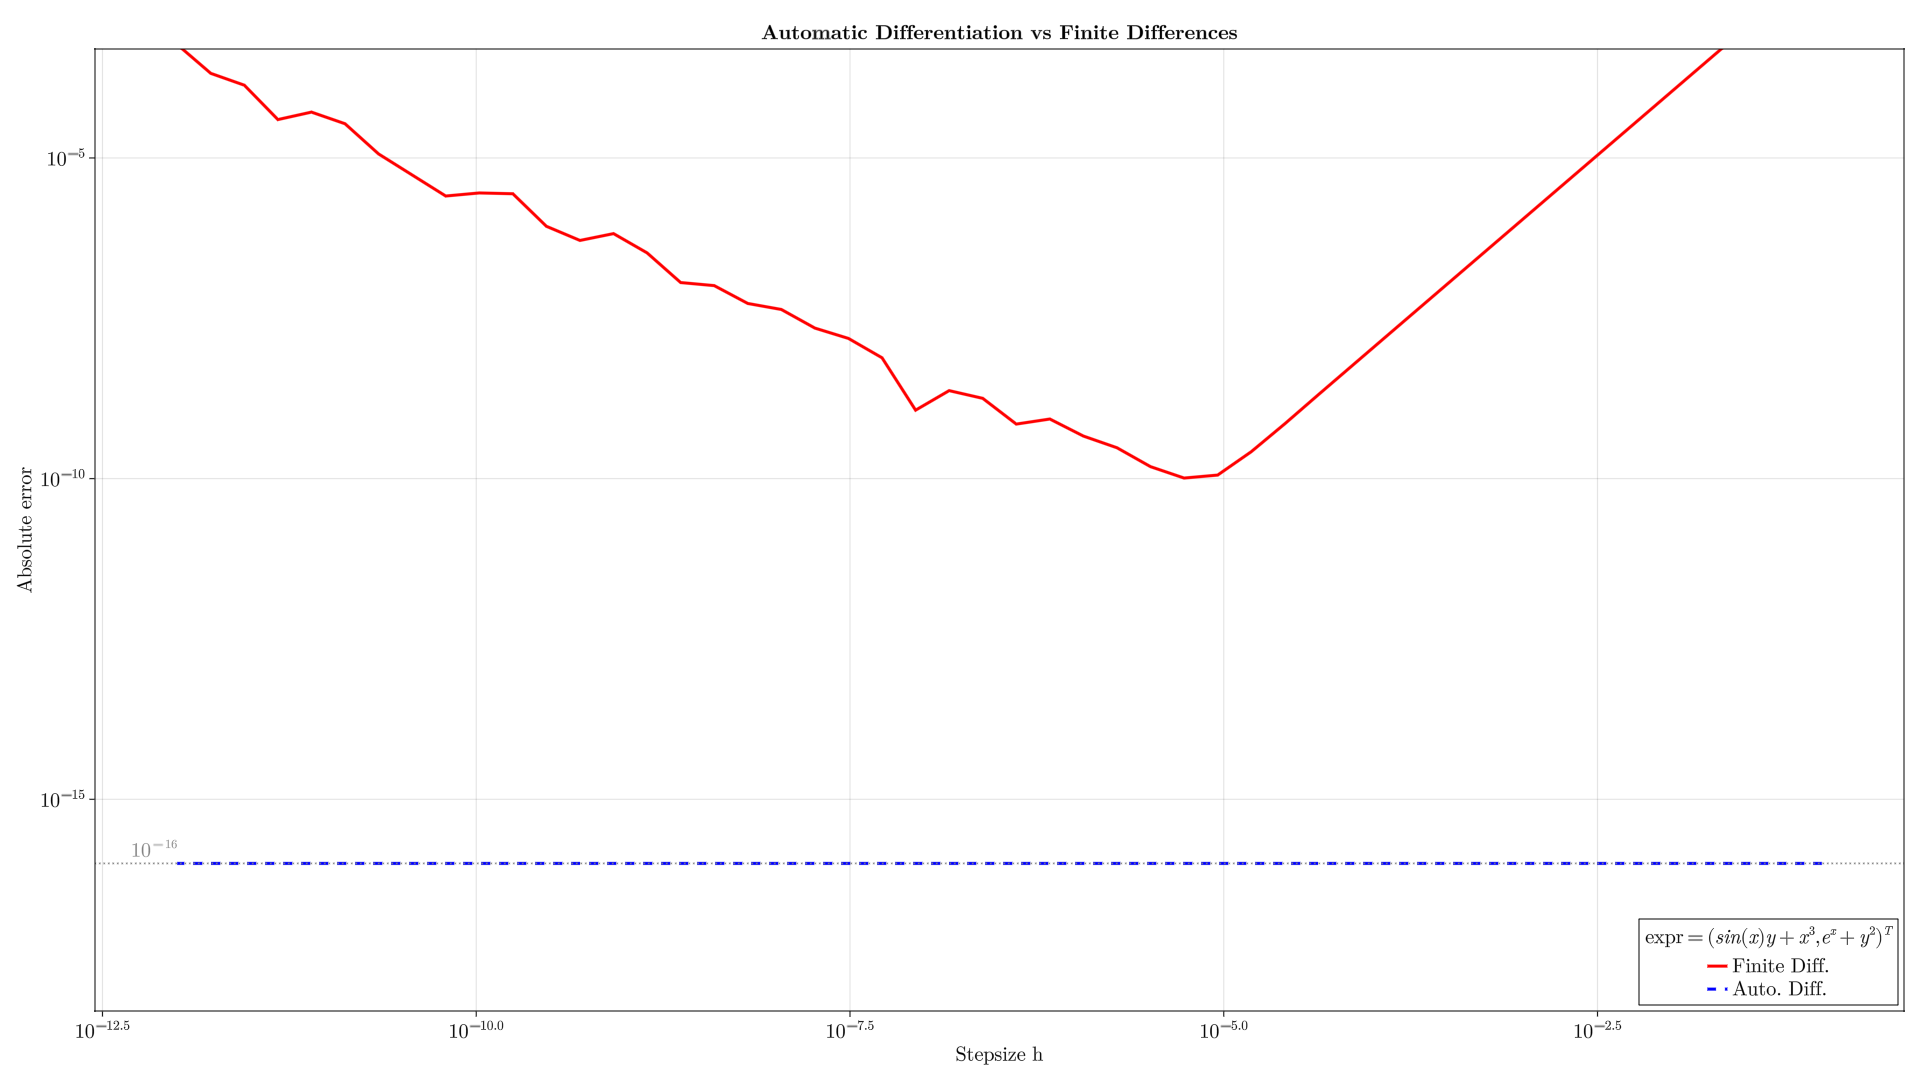
\includegraphics[scale=0.25]{figures/FDvsAD.png}
    \caption{Comparison of the error in computing derivatives using finite differences (red, U-shaped) and automatic differentiation (blue, flat at machine precision).}
    \label{fig:autodiff_vs_fd}
\end{figure}

\section{Geometric Integration via Manifold Projection}

\subsection{The Problem of Invariant Drift}
Standard explicit Runge-Kutta integrators are non-geometric in nature: they do not preserve the algebraic invariants of the phase space. Along a physical null geodesic, the state vector \(\bm{y}\) must remain strictly confined to a sub-manifold \(\mathcal{N}\) embedded in the 8-dimensional phase space. This sub-manifold is defined by the simultaneous vanishing of three invariant constraint functions:
\begin{enumerate}
    \item \textbf{The Lagrangian Null Condition:} \(g_1(\bm{y}) \equiv g_{\mu\nu}(\bm{x}) u^\mu u^\nu = 0\).
    \item \textbf{Conservation of Energy:} \(g_2(\bm{y}) \equiv -(g_{tt}(\bm{x}) u^t + g_{t\phi}(\bm{x}) u^\phi) - E = 0\).
    \item \textbf{Conservation of Axial Angular Momentum:} \(g_3(\bm{y}) \equiv g_{\phi\phi}(\bm{x}) u^\phi + g_{t\phi}(\bm{x}) u^t - L_z = 0\).
\end{enumerate}
During long-term propagation, accumulated floating-point errors drive the unconstrained solution \(\tilde{\bm{y}}\) off this sub-manifold. In strong gravitational environments, even microscopic deviations trigger exponential trajectory divergence.

\subsection{Projection via Lagrange Multipliers}
To suppress this drift, we implement the Manifold Projection method as described in \cite{Hairer2006-te}. Let \(\tilde{\bm{y}}\) denote the provisional state vector computed by the solver at step \(n+1\). We seek a corrected state \(\bm{y}^*\) that satisfies the zero-level constraint equations. Using the method of Lagrange multipliers, we construct the auxiliary objective functional:
\begin{equation}
    \mathcal{S}(\bm{y}^*, \bm{\lambda}) = \frac{1}{2} \|\bm{y}^* - \tilde{\bm{y}}\|^2 + \bm{\lambda}^T \bm{g}(\bm{y}^*),
\end{equation}
Taking the functional gradient with respect to the state vector \(\bm{y}^*\), we obtain:
\begin{equation}
    \bm{y}^* = \tilde{\bm{y}} - \bm{J}(\bm{y}^*)^T \bm{\lambda},
\end{equation}
where \(\bm{J}(\bm{y}) \equiv \frac{\partial \bm{g}}{\partial \bm{y}}\) is the constraint Jacobian matrix. This equation possesses profound geometric meaning: the correction vector \(\delta\bm{y} = \bm{y}^* - \tilde{\bm{y}} = -\bm{J}^T \bm{\lambda}\) lies entirely within the subspace normal to the constraint sub-manifold. Thus, the projection alters the numerical state strictly along directions orthogonal to the physical invariant surface, ensuring the trajectory is not dissipated or artificially damped.

\subsection{Multidimensional Newton-Raphson Iterative Solver}
Substituting the projection equation into the constraint condition yields a non-linear algebraic system for the unknown multipliers \(\bm{\lambda}\). To solve this efficiently, we employ a multidimensional Newton-Raphson scheme. Expanding \(\bm{g}\) in a first-order Taylor series, we define the symmetric Gramian matrix \(\bm{G} \equiv \bm{J} \bm{J}^T \in \mathbb{R}^{3 \times 3}\). The iterative Newton increment \(\Delta \bm{\lambda}^{(k)}\) is computed via:
\begin{equation}
    \bm{G} \, \Delta \bm{\lambda}^{(k)} = \bm{g}(\bm{y}^{(k)}) \quad \implies \quad \Delta \bm{\lambda}^{(k)} = \bm{G}^{-1} \bm{g}(\bm{y}^{(k)}).
\end{equation}
The step-by-step execution flow of the Manifold Projection proceeds as follows:
\begin{enumerate}
    \item \textbf{Initialization:} Set \(\bm{\lambda}^{(0)} = \bm{0}\) and \(\bm{y}^{(0)} = \tilde{\bm{y}}\). Evaluate \(\bm{J}\) using the exact forward-mode AD introduced in Section 2.3.
    \item \textbf{Iterative Correction Loop:} For \(k = 1, 2, \dots\):
    \begin{align}
        \bm{u}^{(k)} &= \tilde{\bm{y}} + \bm{J}^T \bm{\lambda}^{(k)}, \\
        \bm{R}^{(k)} &= \bm{g}(\bm{u}^{(k)}), \\
        \Delta \bm{\lambda}^{(k)} &= -\bm{G}^{-1} \bm{R}^{(k)}, \\
        \bm{\lambda}^{(k+1)} &= \bm{\lambda}^{(k)} + \Delta \bm{\lambda}^{(k)}.
    \end{align}
    \item \textbf{Convergence Criterion:} Terminate the loop when the increment norm satisfies:
    \begin{equation}
        \|\Delta \bm{\lambda}^{(k)}\| < \text{tol},
    \end{equation}
    where we set the tolerance to a constant value equal to the machine precision limit, \(\text{tol} = 10^{-16}\). 
    \begin{quote}
    \textit{We note that while a step-dependent tolerance, \(\text{tol} = c \cdot \Delta t^{p+1}\), could be adopted to reduce the number of Newton-Raphson iterations during large integration steps, we have deliberately chosen a fixed, extremely strict tolerance of \(10^{-16}\). This choice does not alter the underlying physics or the mathematical formulation of the projection, but ensures that the state vector is re-projected onto the constraint sub-manifold with the absolute maximum accuracy achievable by the machine, regardless of the local step size. Consequently, the only cost incurred is an increase in computational power, which is negligible compared to the total ODE integration time, while completely guaranteeing the conservation of all physical quantities.}
    \end{quote}
    To safeguard against potential infinite loops in the event of numerical singularities (e.g., extremely close to the Boyer-Lindquist coordinate singularity), we additionally set a maximum limit of 500 iterations, possibly sacrificing some accuracy.
    \item \textbf{State Replacement:} Overwrite the integrator state with \(\bm{y}^*\) and evaluate the termination triggers.
\end{enumerate}

\subsection{Convergence of the Newton--Raphson Iteration}
The projection reduces to solving $\bm{F}(\bm{\lambda}) \equiv
\bm{g}\!\left(\tilde{\bm{y}} + \bm{J}^{T}\bm{\lambda}\right) = \bm{0}$, whose exact
Jacobian is $\bm{F}' = \bm{J}\bm{J}^{T} \equiv \bm{G}$. The multidimensional
Newton--Raphson method enjoys the following classical guarantee.

\paragraph{Theorem (quadratic convergence).}
\emph{Let $\bm{F} \in C^2$, $\bm{F}(\bm{\lambda}_*) = \bm{0}$, and $\bm{G}(\bm{\lambda}_*)$ nonsingular. Then for $\bm{\lambda}_0$ sufficiently close to $\bm{\lambda}_*$ the
iteration converges and}
\begin{equation}
    \|\bm{\lambda}_{k+1} - \bm{\lambda}_*\| \;\le\;
    \frac{M_2}{2\,\sigma_{\min}}\,
    \|\bm{\lambda}_k - \bm{\lambda}_*\|^2 ,
\end{equation}
\emph{where $M_2$ bounds $\|\bm{F}''\|$ and $\sigma_{\min}$ is the smallest singular
value of $\bm{G}(\bm{\lambda}_*)$.}

The proof is a second-order Taylor expansion of $\bm{F}(\bm{\lambda}_k)$ about
 $\bm{\lambda}_*$: the linear terms cancel exactly by construction of the Newton step,
leaving a residual quadratic in the error --- the number of correct digits roughly
doubles per iteration, which is why the observed iteration counts are tiny whenever
 $\tilde{\bm{y}}$ is already close to the constraint manifold (i.e.\ always, when the
integrator is accurate). Two practical refinements have a precise theory. First,
\emph{freezing} the Jacobian ($\tilde{\bm{G}} = \bm{G}$ held fixed) yields the chord
method, which converges only linearly, with rate $\rho = \|\bm{I} -
\tilde{\bm{G}}^{-1}\bm{G}\|$; periodically recomputing $\bm{G}$ restores the full
quadratic rate. This is the exact trade-off exploited when the Jacobian refresh is
amortized over several iterations: the projection is dominated by the cost of the
constraint Jacobian, and the refresh cadence converts a per-iteration cost into a
per-$K$-iteration cost at negligible loss of convergence speed. Second, since
 $\bm{G}$ is symmetric positive semidefinite, it is positive definite --- and the
linear system uniquely solvable --- iff $\bm{J}$ has full row rank $m = 3$.

\subsection{Regularity of the Constraints}
The Lagrange construction presumes that the three constraint gradients
 $\partial_{\bm{y}} g_1, \partial_{\bm{y}} g_2, \partial_{\bm{y}} g_3$ are linearly
independent on a neighbourhood of the constraint manifold $\mathcal{N}$. This is
generically the case: $\mathrm{d}E$ and $\mathrm{d}L_z$ are the contractions with the
mutually independent Killing covectors $\xi_\mu$ and $\eta_\mu$, and the null
constraint gradient $g_{\mu\nu}u^\nu$ is not a linear combination of them at any
physical point of phase space. By the implicit function theorem the projection is then
locally unique and depends smoothly on $\tilde{\bm{y}}$. Near $r = r_+$ the metric
derivatives entering $\bm{J}$ diverge as $1/\Delta$; the constraints remain regular
(their defining functions stay finite) but the Newton system becomes
ill-conditioned, which is why a maximum-iteration safeguard accompanies the solver.
This degradation is confined to a region from which no observable photon escapes, so it cannot contaminate the image.

\subsection{Projection Versus Alternative Stabilization Strategies}
Projection belongs to the broader family of \emph{geometric integrators}, which are
designed to respect structure of the flow rather than only its pointwise accuracy. The
alternatives are instructive to contrast:
\begin{enumerate}
    \item \textbf{Constraint damping (Baumgarte stabilization):} augment the vector
    field with terms that exponentially pull the solution back to $\mathcal{N}$. This
    modifies the equations actually integrated and introduces a free damping time
    scale; the invariants are restored only approximately and at the price of
    systematically perturbing the dynamics.
    \item \textbf{Phase-space reduction:} eliminate degrees of freedom by solving the
    constraints analytically (e.g.\ determining $u^t$ from the null condition). Exact
    by construction, but the reduced system loses the symmetries that make adaptive
    control and error estimation uniform across the phase space, and it is
    metric-specific --- precisely what a general-purpose tracer must avoid.
    \item \textbf{Symplectic integrators:} for Hamiltonian systems they conserve a
    modified Hamiltonian over exponentially long times (backward error analysis),
    giving superb long-term energy behaviour. However, geodesic Hamiltonians are
    non-separable in general coordinates (forcing implicit methods), adaptive step
    sizes destroy the symplectic property, and symplecticity preserves a \emph{nearby}
    energy rather than the exact invariants $E$, $L_z$ demanded here.
\end{enumerate}
Projection is distinguished by three properties that make it the method of choice for
ray tracing: it is \emph{exact} (the invariants hold to machine precision at every
accepted step, with no secular drift), \emph{unbiased} (the correction lies entirely
in the normal space to $\mathcal{N}$, so the tangential, physical dynamics is that of
the underlying integrator to its full order, no order reduction occurs), and
\emph{parameter-free} (no damping constants, no reduced coordinates). For reversible
problems one may additionally symmetrize the projection to inherit long-term
reversibility; for the present purpose the standard projection suffices, since the
observables are fixed by the invariant values and the tangential accuracy, both of
which are controlled as described above.

\section{High-Order Adaptive Integration}
\subsection{Butcher Structure and Order Conditions}
An explicit $s$-stage Runge--Kutta method is specified by its Butcher tableau:
\begin{equation}
    \bm{k}_i = \bm{f}\!\left(\bm{y}_n + h\sum_{j=1}^{i-1} a_{ij}\,\bm{k}_j\right),
    \qquad
    \bm{y}_{n+1} = \bm{y}_n + h\sum_{i=1}^{s} b_i\, \bm{k}_i .
\end{equation}
Matching the Taylor expansion of $\bm{y}_{n+1}$ with that of the exact solution through
order $p$ imposes a set of algebraic \emph{order conditions}, one per rooted tree;
their number grows as $1, 2, 4, 8, 17, 37, 78, 167$ for $p = 1, \dots, 8$. The
combinatorial explosion explains both why very high orders require many stages and why
the construction of efficient coefficients (as in Verner's embedded pairs) is a
non-trivial numerical-analysis achievement. For geodesic integration the right-hand
side is analytic (away from $\Delta = 0$), so high order pays off without the
order-reduction pathologies familiar from stiff or non-smooth problems.

\subsection{Embedded Pairs and Local Error Estimation}
Practical step-size control requires an error estimate per step. An \emph{embedded
pair} shares the internal stages $\bm{k}_i$ between two solutions of orders $p$ and
 $p - 1$,
\begin{equation}
    \bm{y}_{n+1} = \bm{y}_n + h\sum_i b_i \bm{k}_i, \qquad
    \hat{\bm{y}}_{n+1} = \bm{y}_n + h\sum_i \hat{b}_i \bm{k}_i,
    \qquad
    \bm{e}_{n+1} = \bm{y}_{n+1} - \hat{\bm{y}}_{n+1} \approx \mathcal{O}(h^{p}),
\end{equation}
so the difference $\bm{e}_{n+1}$ estimates the error of the \emph{lower}-order result
at negligible extra cost, and the higher-order result is propagated (local
extrapolation). The scalar error measure is taken in a component-wise weighted norm,
\begin{equation}\label{eq:weighted_err}
    \mathrm{err} = \max_i\;
    \frac{\big|\,(\bm{e}_{n+1})_i\,\big|}{\mathrm{atol} + \mathrm{rtol}\cdot
    \max\!\left(|y_i|,\,|\hat{y}_i|\right)} ,
\end{equation}
which makes the tolerance scale-invariant across state components of disparate
magnitude (here: coordinates versus four-velocity components).

\chapter{Setup}

Having established the theoretical framework of stationary axisymmetric spacetimes and the geodesic equations governing null trajectories, we now proceed to describe the algorithms deployed to perform the black hole imaging.

\section{Backward Ray Tracing and Initial Conditions}

To generate images of the shadow and the surrounding strongly lensed region, we adopt a backward ray-tracing paradigm. Unlike the standard forward approach, where photons are emitted from a source and tracked towards an observer, backward ray-tracing treats each pixel of the observer's screen as an independent initial condition for a null geodesic. This is possible due to the fact that, in the absence of scattering, light rays are reversible. 

\subsection{Choice of Coordinate System}
We begin by defining the observer's position. In our framework, we work any coordinates spherical \((t, r, \theta, \phi)\) or Cartesian \(t,x,y,z\), since our methodology allows for any metric expressed in any coordinate system. Our AD machinery alongside the geometric high-order integration scheme we use allow us to do so. Thus, our testbed became the Kerr black hole since it allows both coordinate expression (Boyer-Lindquist and Kerr-Schild) as well as the static Schwarzschild counterpart by setting $a=0$.

In every case, there exists an event horizon which we need to deal with numerically. Therefore, our integrations are terminated at a radial distance of approximately \(r \approx 1.15 M\) to \(1.3 M\) (depending on the case), ensuring that the physical quantities remain well-defined and machine-precision accuracy is strictly maintained before the coordinate breakdown occurs.

\subsection{Grid Construction and Initial Conditions}
The observer is assumed to be located at a fixed radial distance \(r_0 \gg M\) and at an inclination angle \(\theta_0\) relative to the black hole's spin axis. The initial position vector is given by:
\begin{equation}
    \bm{x}_{\text{obs}} = (t_0, r_0, \theta_0, \phi_0),
\end{equation}
where we typically set \(t_0 = 0\) and \(\phi_0 = \pi/2\) for simplicity. 

We then construct a two-dimensional grid of initial conditions \(N \times M\), where \(N\) and \(M\) correspond to the number of different values for our two impact parameters \(b\) and \(\alpha\), respectively. These parameters define the apparent position of the ray on the observer's celestial sphere and are linearly mapped to the grid's horizontal and vertical axes.

For each point \((b_i, \alpha_j)\) on this grid, we construct the initial four-velocity \(\bm{u}^\mu\). To ensure that the photons are physical (massless), we enforce the null condition via the normalization of the initial four-momentum:
\begin{equation}
    g_{\mu\nu} u^\mu u^\nu = 0.
\end{equation}
In practice, this is achieved by taking an unnormalized spatial velocity vector, solving for the time component of the velocity that satisfies the null condition, and scaling it appropriately. The conserved energy \(E\) and axial angular momentum \(L_z\) are calculated directly from the metric tensor at the observer's location.

\subsection{UV Mapping and Calibration}

To generate an image, we place a virtual camera at a fixed radial distance \(r_0\) and inclination angle \(\theta_0\). We map the impact parameters \((b, \alpha)\) onto the two-dimensional observer's screen, forming a grid \(N \times M\) of initial conditions. For every pixel, the photon is traced backwards as described before.


For photons that escape to infinity, we map their final angular coordinates \((\theta, \phi)\) onto an equirectangular background image. The mapping is given by:
\begin{align}
    u &= 1 - \frac{\mod(\phi - \pi, 2\pi)}{2\pi}, \\
    v &= \frac{\mod(\theta, \pi)}{\pi},
\end{align}
where \((u, v)\) correspond to the normalized horizontal and vertical pixel coordinates of the background image. To ensure the correctness of this mapping and the proper handedness of the celestial sphere, we perform a rigorous calibration step using a dedicated four-colour test image (with distinct quadrants of red, green, blue, and yellow). By verifying the correct orientation of the colours in the rendered shadow, we guarantee that our subsequent simulations using realistic Milky Way backgrounds produce physically accurate gravitational lensing. However different choices of tghe UV mapping result in different outputs and thus conventions.

\begin{figure}[H]
    \centering
    
\includegraphics[width=0.4\textwidth]{figures/test_image.jpg}
    \caption{Four-colour calibration image used to verify the UV mapping and handedness of the celestial sphere projection.}
    \label{fig:test_image}
\end{figure}

\chapter{Results}

\section{Validation of Numerical Stability}

Before presenting the physical results and the astrophysical imaging, we systematically validate the robustness of our proposed numerical integrator. The primary objective of this section is to demonstrate that the coupling of the high-order adaptive Runge-Kutta scheme with the Manifold Projection technique successfully constrains the drift of the conserved quantities to machine precision, even for highly unstable or long-lived photon trajectories.

Furthermore, we demonstrate the effectiveness of the projection algorithm through a controlled pedagogical example of circular motion. We integrate a simple harmonic oscillator constrained to a unit circle in the Euclidean plane, using a standard 4th-order Runge-Kutta scheme with a fixed step size. Without projection, the unconstrained solution spirals outwards, accumulating energy. With the implementation of the Manifold Projection, the orbit remains exactly on the circle indefinitely, illustrating the general applicability of the method. The success of this simple example confirms the mathematical robustness of the projection algorithm we have implemented for the relativistic case.

\begin{figure}[H]
    \centering
    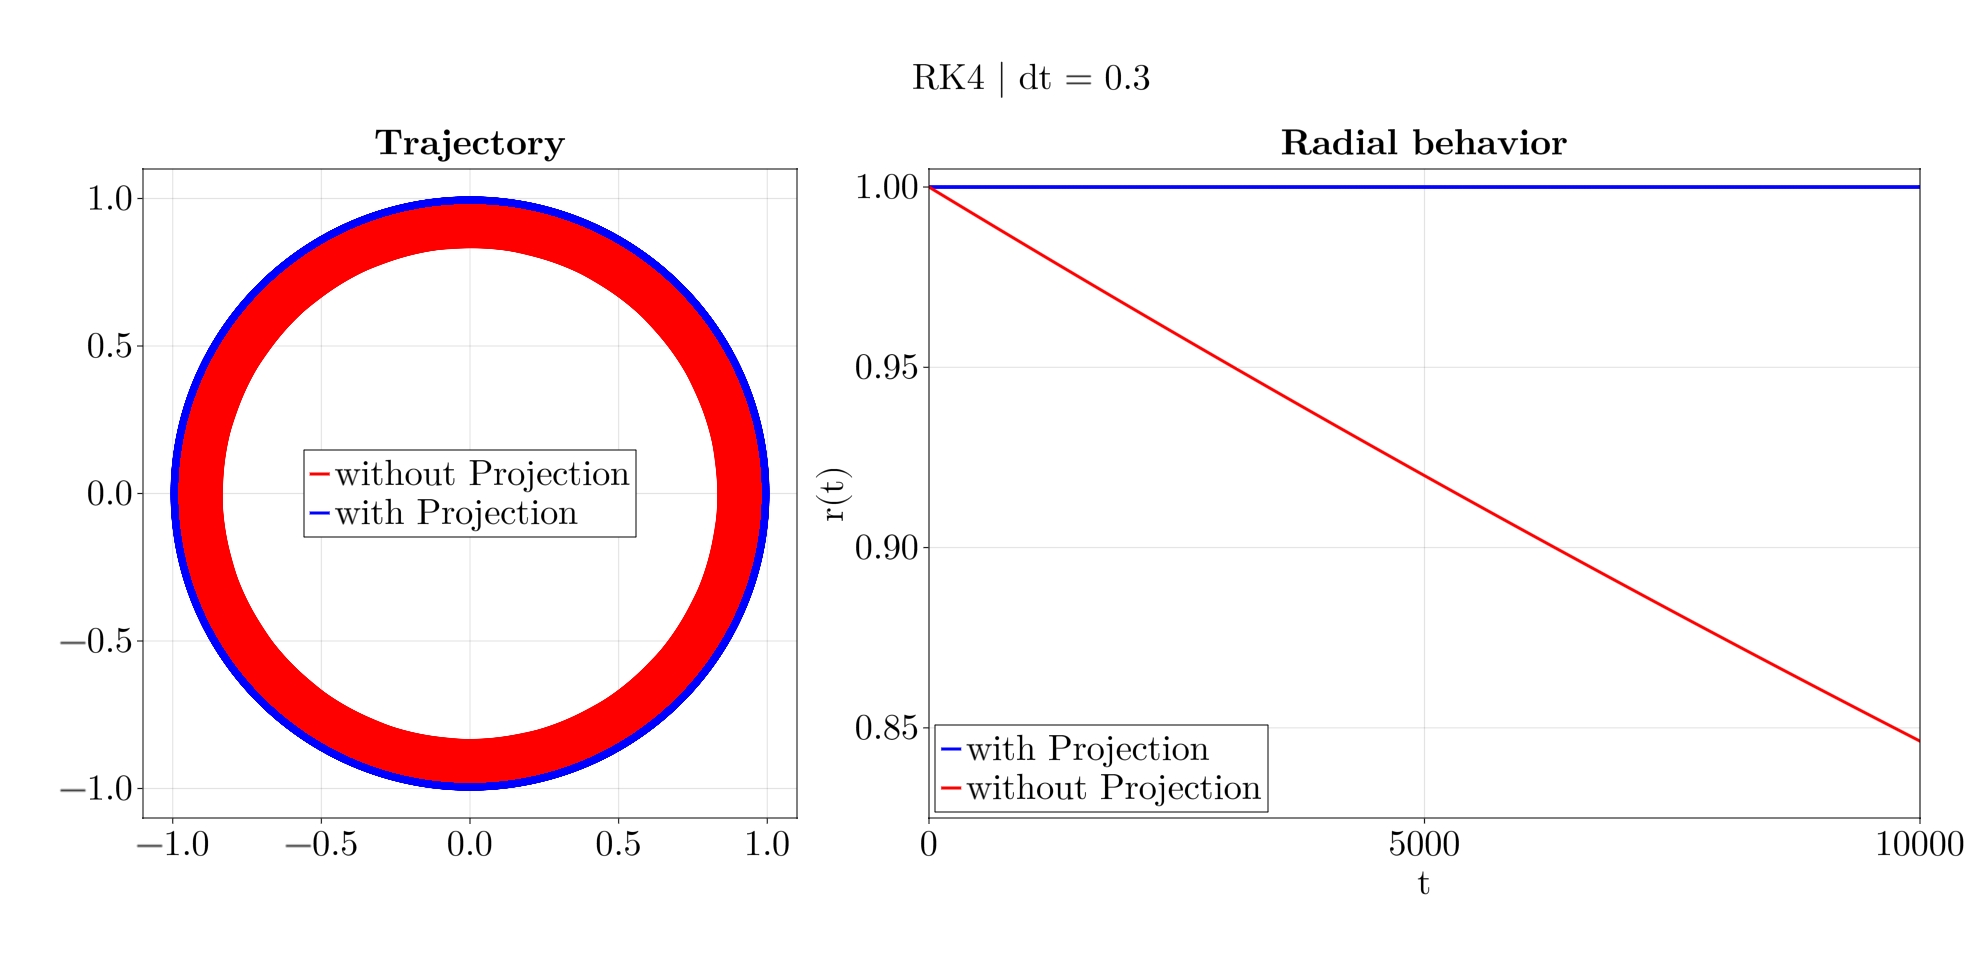
\includegraphics[width=0.8\textwidth]{figures/manifold_projection_static.png}
    \caption{The ODE used for this figure is $\dot{x}=y, \dot{y}=-x$, thus the analytical solution is just a circle.
    \textbf{Top}: The trajectory of the same initial condition using the typical RK4 using the manifold projection (blue) and without (red). \textbf{Middle and Bottom}: the behavior of the radius in time for the two cases we compare.}
    \label{fig:errors_projection}
\end{figure}

Our findings are presented in Fig.~\ref{fig:errors_projection}. In the absence of the geometric projection (red curve), the unconstrained integration leads to a systematic accumulation of truncation and round-off errors. While the trajectory may initially appear accurate, the errors in the conserved quantity grows significantly over time. On the contrary, the geometric integration technique (blue curve) preserves the expected behavior exactly. Moreso, this happens even in an almost trivial right-hand side expression. This numerical drift is particularly severe in our main problem, i.e. when the photons approach the unstable photon sphere, where the highly non-linear behaviour of the metric amplifies these deviations, eventually leading to unphysical trajectories.

\subsection{Fundamental Photon Orbits and Dynamics}

Now moving on to the relativistic trajectories in the near extremal ($a=0.998$) Kerr manifold, we monitor the evolution of the relative errors in the conserved energy $\Delta e / e_0$, the axial angular momentum $\Delta l / l_0$, and the error in the null constraint $g_{\mu\nu}u^\mu u^\nu$, along the affine parameter $\lambda$. 


Figures \ref{fig:err2}, \ref{fig:err3} and \ref{fig:err3} demonstrate the effectiveness of our method, and the layout is the following
\begin{itemize}[align=left]
    \item[\textbf{Top Left}:] 
    {On the top left we see the behavior of the radius as a percentage of the initial one,in order to show that there is no sudden jump (either ejection or plunge to the singularity)}.
    \item[\textbf{Top Middle}:] The radius.
    
    \item[\textbf{Top Right}:] The full 3D trajectory of the evolution.
    \item[\textbf{Bottom Left}:] The relative error of the energy for each step.
    \item[\textbf{Bottom Middle}:] The relative error of the angular momentum.
    \item[\textbf{Bottom Right}:] The null condition error.
\end{itemize}


\subsection{Scattering Orbits}
For values of the impact parameter satisfying \(|b| > b_c\), the effective potential \(V_{\text{eff}}\) prevents the photon from crossing the centrifugal barrier. The photon approaches the black hole, reaches a minimum radial distance \(r_{\min} > r_{\text{ph}}\), and subsequently escapes to spatial infinity. This behaviour gives rise to the characteristic "V" shape in the radial coordinate as a function of the affine parameter, \(r(\lambda)\), which we display in Fig. \ref{fig:err2}. 

This class of orbits is particularly relevant for studies of gravitational lensing. The exact radius of closest approach, \(r_{\min}\), depends sensitively on the impact parameter and the black hole's spin. By resolving these trajectories to machine precision, our framework accurately captures the strong deflection experienced by photons passing in the vicinity of the photon sphere.

\begin{figure}[H]
    \centering
    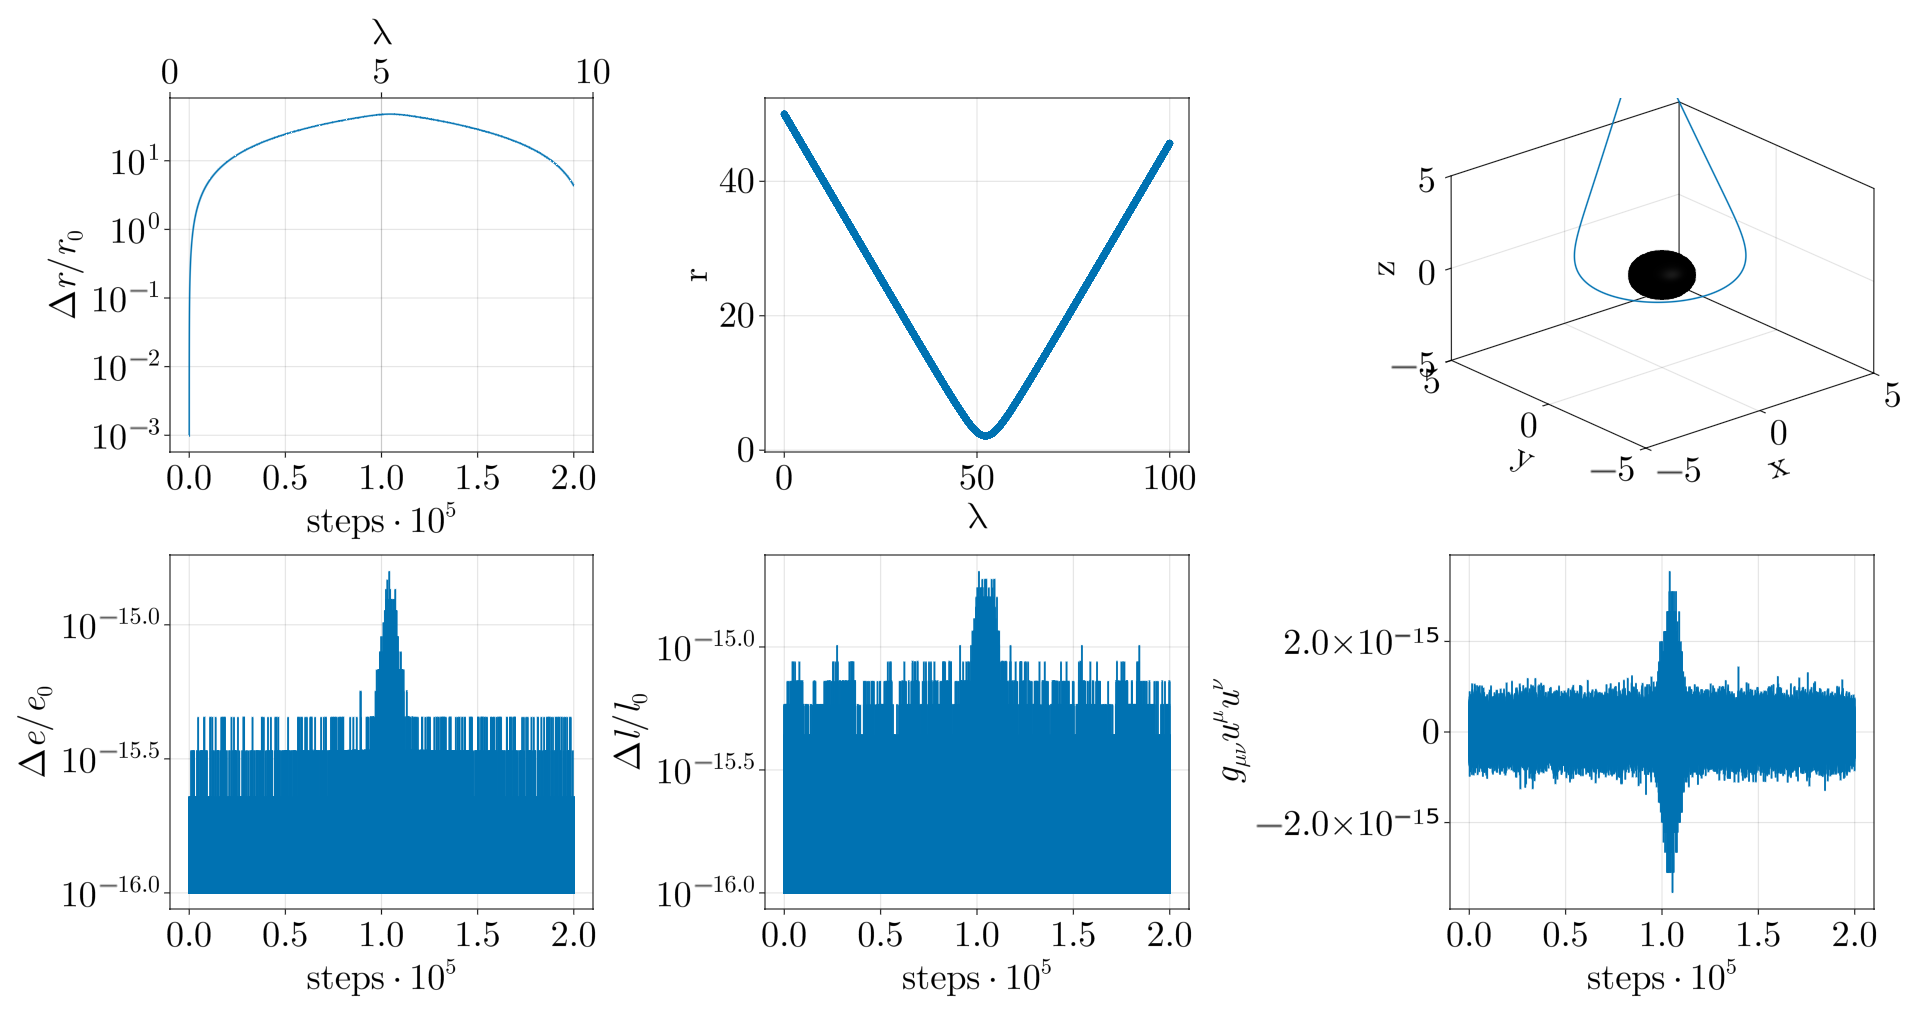
\includegraphics[width=0.9\linewidth]{figures/errors_V.png}
    \caption{Scattering orbit.}
    \label{fig:err2}
\end{figure}

\subsection{Bound Spiral Orbits (Transient Capture)}
In the limit where the impact parameter approaches the critical value (\(|b| \rightarrow b_c\)), the photon can orbit the black hole multiple times in the vicinity of the unstable photon sphere before either plunging into the event horizon or escaping to infinity. These transient capture orbits are inherently unstable, characterized by an exponential sensitivity to initial conditions, governed by the Lyapunov exponent of the spacetime.

Because of this extreme sensitivity, the accurate numerical integration of these orbits represents one of the most stringent tests of our Manifold Projection algorithm. Any microsecond of numerical drift or round-off error would artificially eject the photon from its bound trajectory. Figure \ref{fig:err1} demonstrates that our algorithm maintains the invariants below the \(10^{-12}\) threshold even after falling in the black hole, after staying in a highly unstable region, allowing us to precisely resolve the number of windings before the photon eventually escapes or is captured.

\begin{figure}[H]
    \centering
    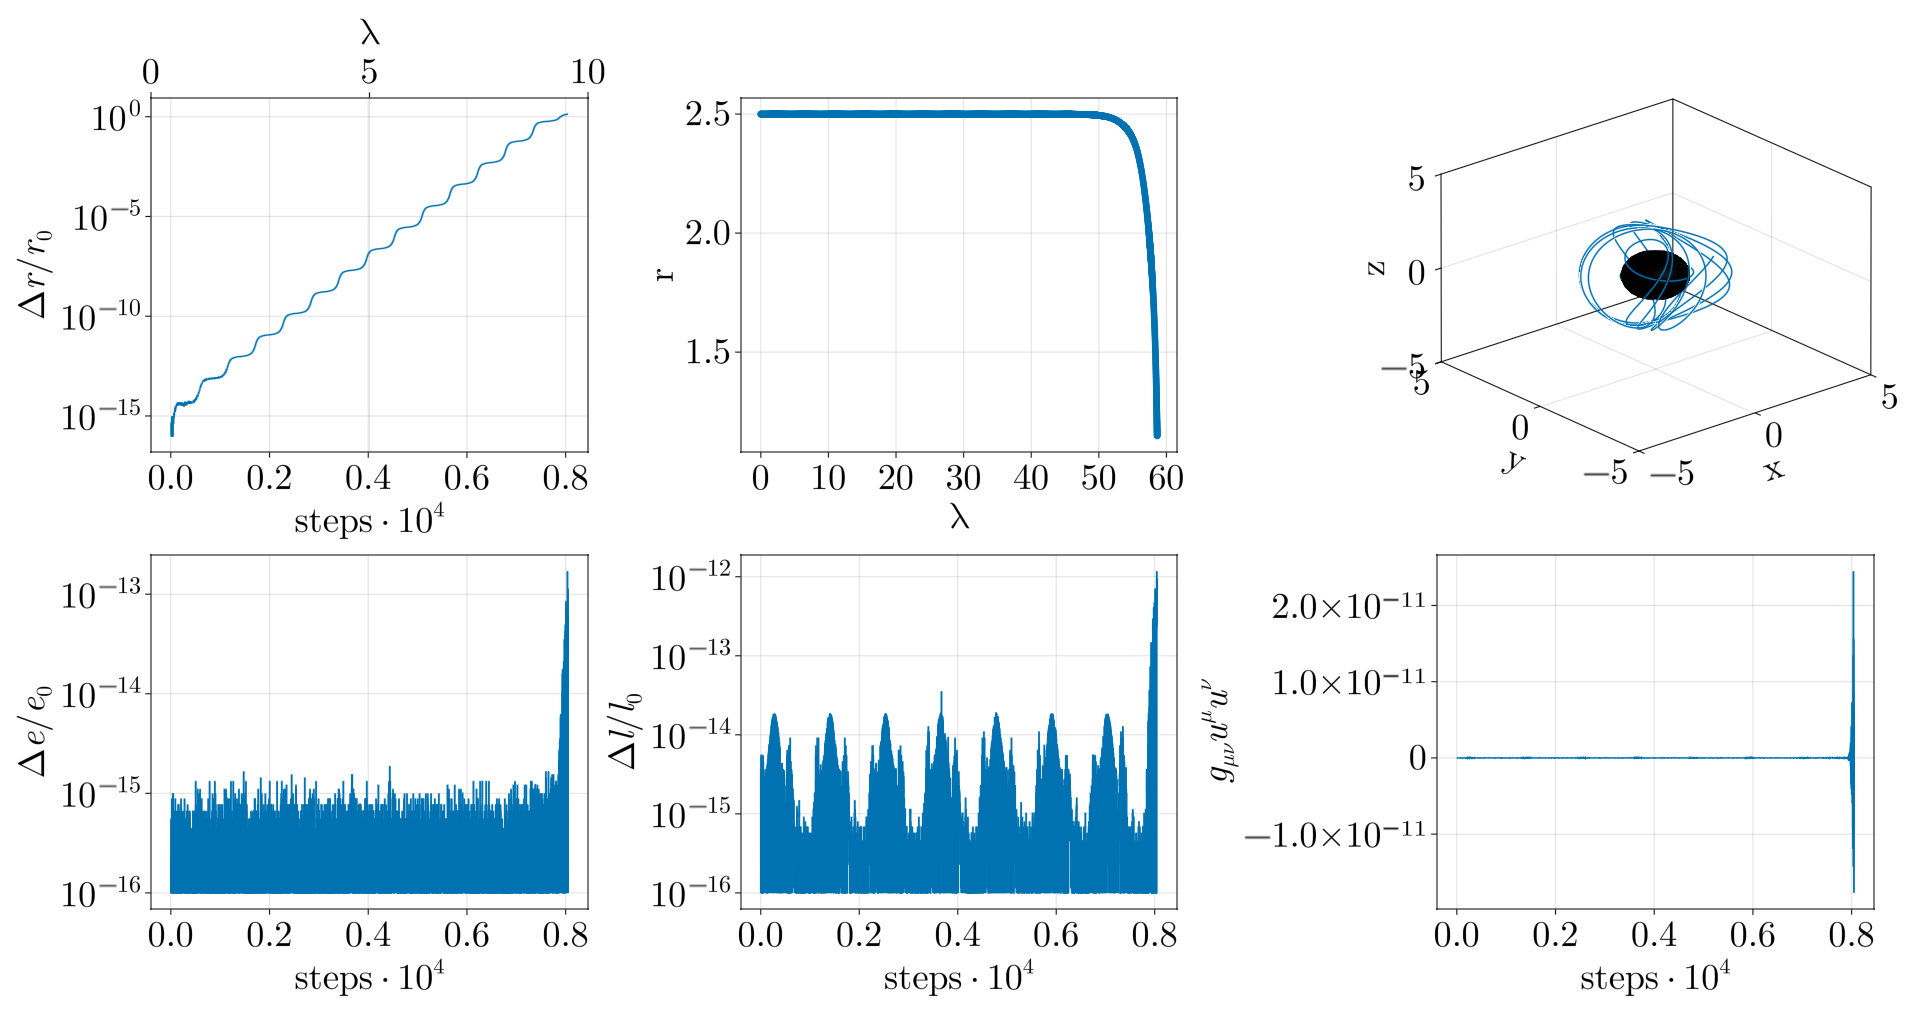
\includegraphics[width=0.9\linewidth]{figures/errors_stable.png}
    \caption{(Almost) bound spiral orbit with a final capture.}
    \label{fig:err1}
\end{figure}

\subsection{Direct Capture Orbits}
Finally, for impact parameters satisfying \(|b| < b_c\), the photon lacks sufficient angular momentum to overcome the effective potential barrier. It plunges inwards, with the radial coordinate \(r(\lambda)\) monotonically decreasing until it crosses the event horizon at \(r = r_+\). 

In our ray-tracing framework, these photons will correspond to the dark pixels of the black hole shadow. Their trajectories terminate when the radial coordinate reaches (near) the horizon, at which point the integration is halted. The robustness of the projection ensures that the energy and angular momentum remain conserved even during this rapid infall, preventing unphysical numerical oscillations near the coordinate singularity.

\begin{figure}[H]
    \centering
    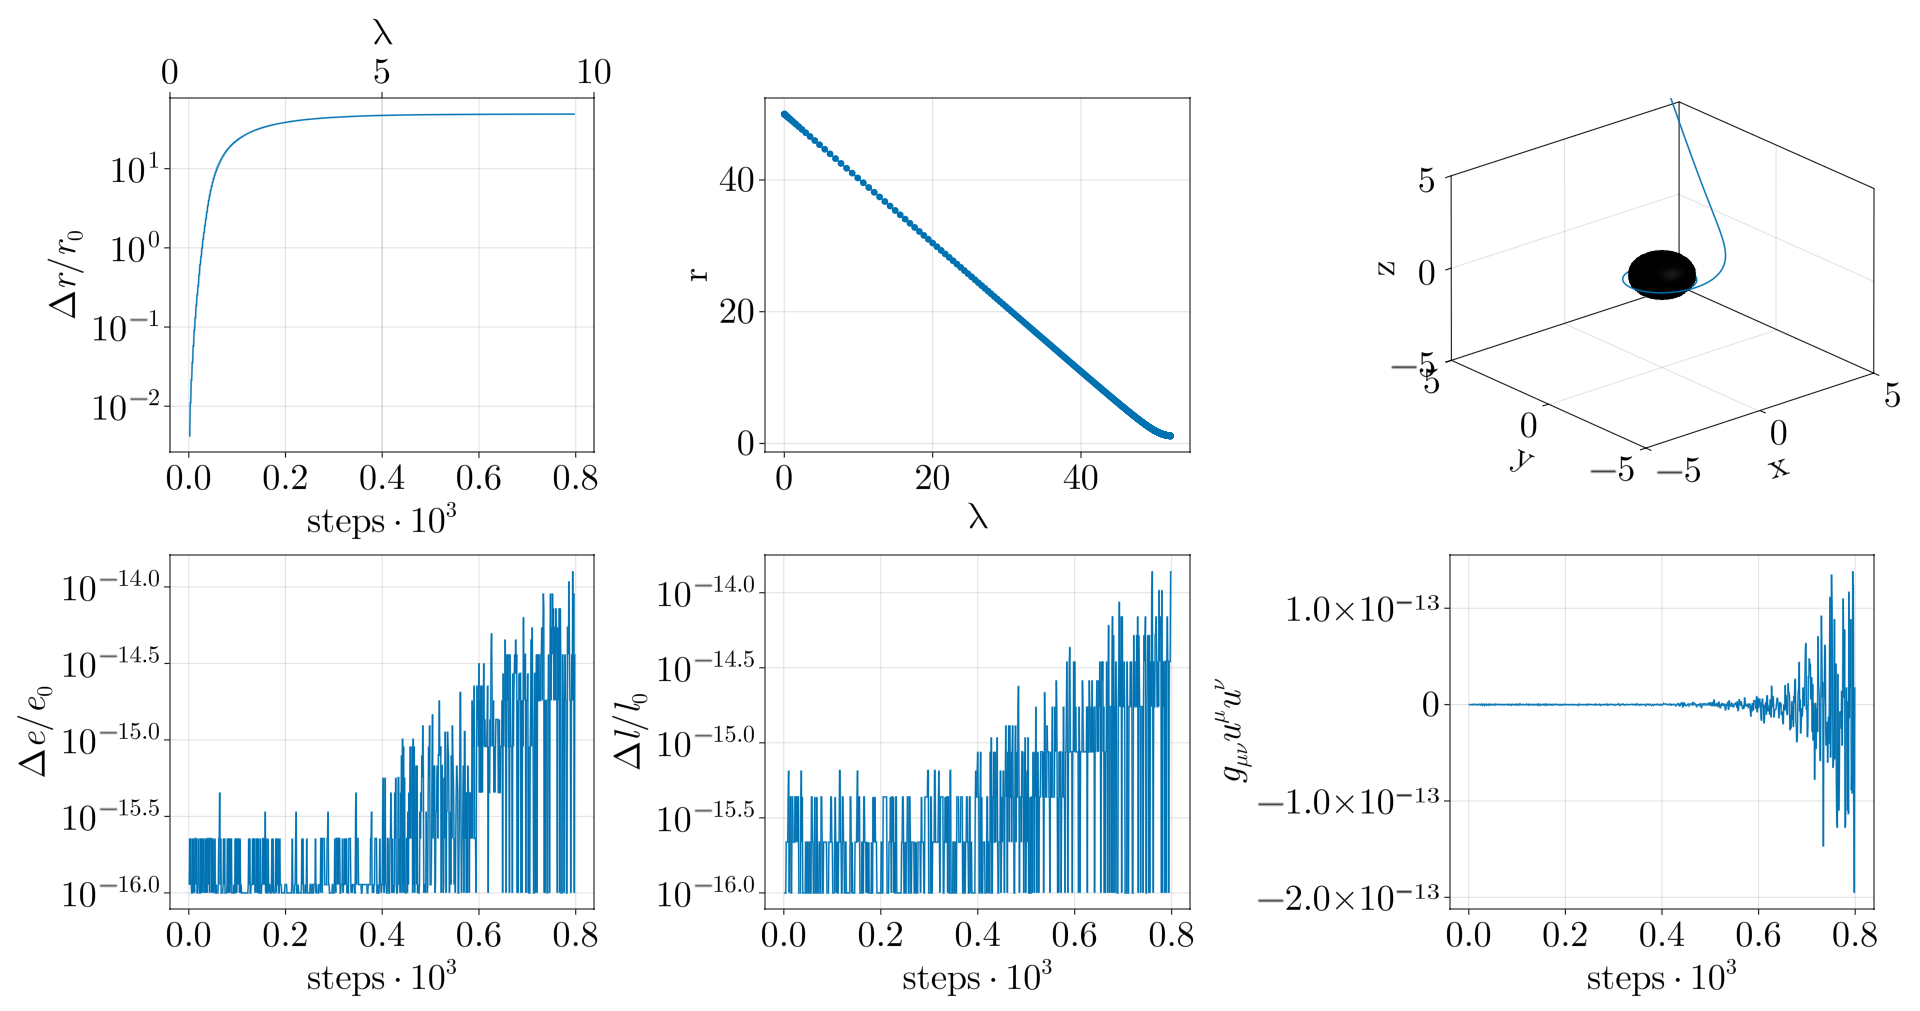
\includegraphics[width=0.9\linewidth]{figures/errors.png}
    \caption{Direct capture.}
    \label{fig:err3}
\end{figure}
Finally, these three fundamental trajectory classes provide the complete mapping between the observer's impact parameters and the resulting image structure. They form the underlying physical basis for the astrophysical imaging we present in the following section. Moreover we have now proved that our method is capable to deal with all of them indiscriminately.

\section{Black Hole Shadow and Astrophysical Imaging}

Having systematically classified and resolved the fundamental photon orbits, we now proceed to construct the images of the black hole as seen by a distant observer. This bridges the gap between the theoretical geodesic structure and observable astrophysical signatures, a key objective of modern strong-field gravity research.
\subsection{Gravitational Lensing of a Point Source}
\label{sec:point_source_lensing}

Before proceeding to complex astrophysical backgrounds and continuous accretion disks, we validate the imaging capabilities of our framework by simulating the gravitational lensing of a simple, monochromatic point source. This scenario serves as a stringent, isolated test of the code's ability to resolve the extreme light bending and the exponential sensitivity of photon trajectories in the strong-field regime, free from the complexities of radiative transfer models.

We place a point source (represented as a red dot) directly behind the black hole relative to the distant observer. The resulting lensed image, presented in Fig.~\ref{fig:point_source_lensing}, reveals the rich and highly non-linear topology of strong-field gravitational lensing.

\begin{figure}[H]
    \centering
    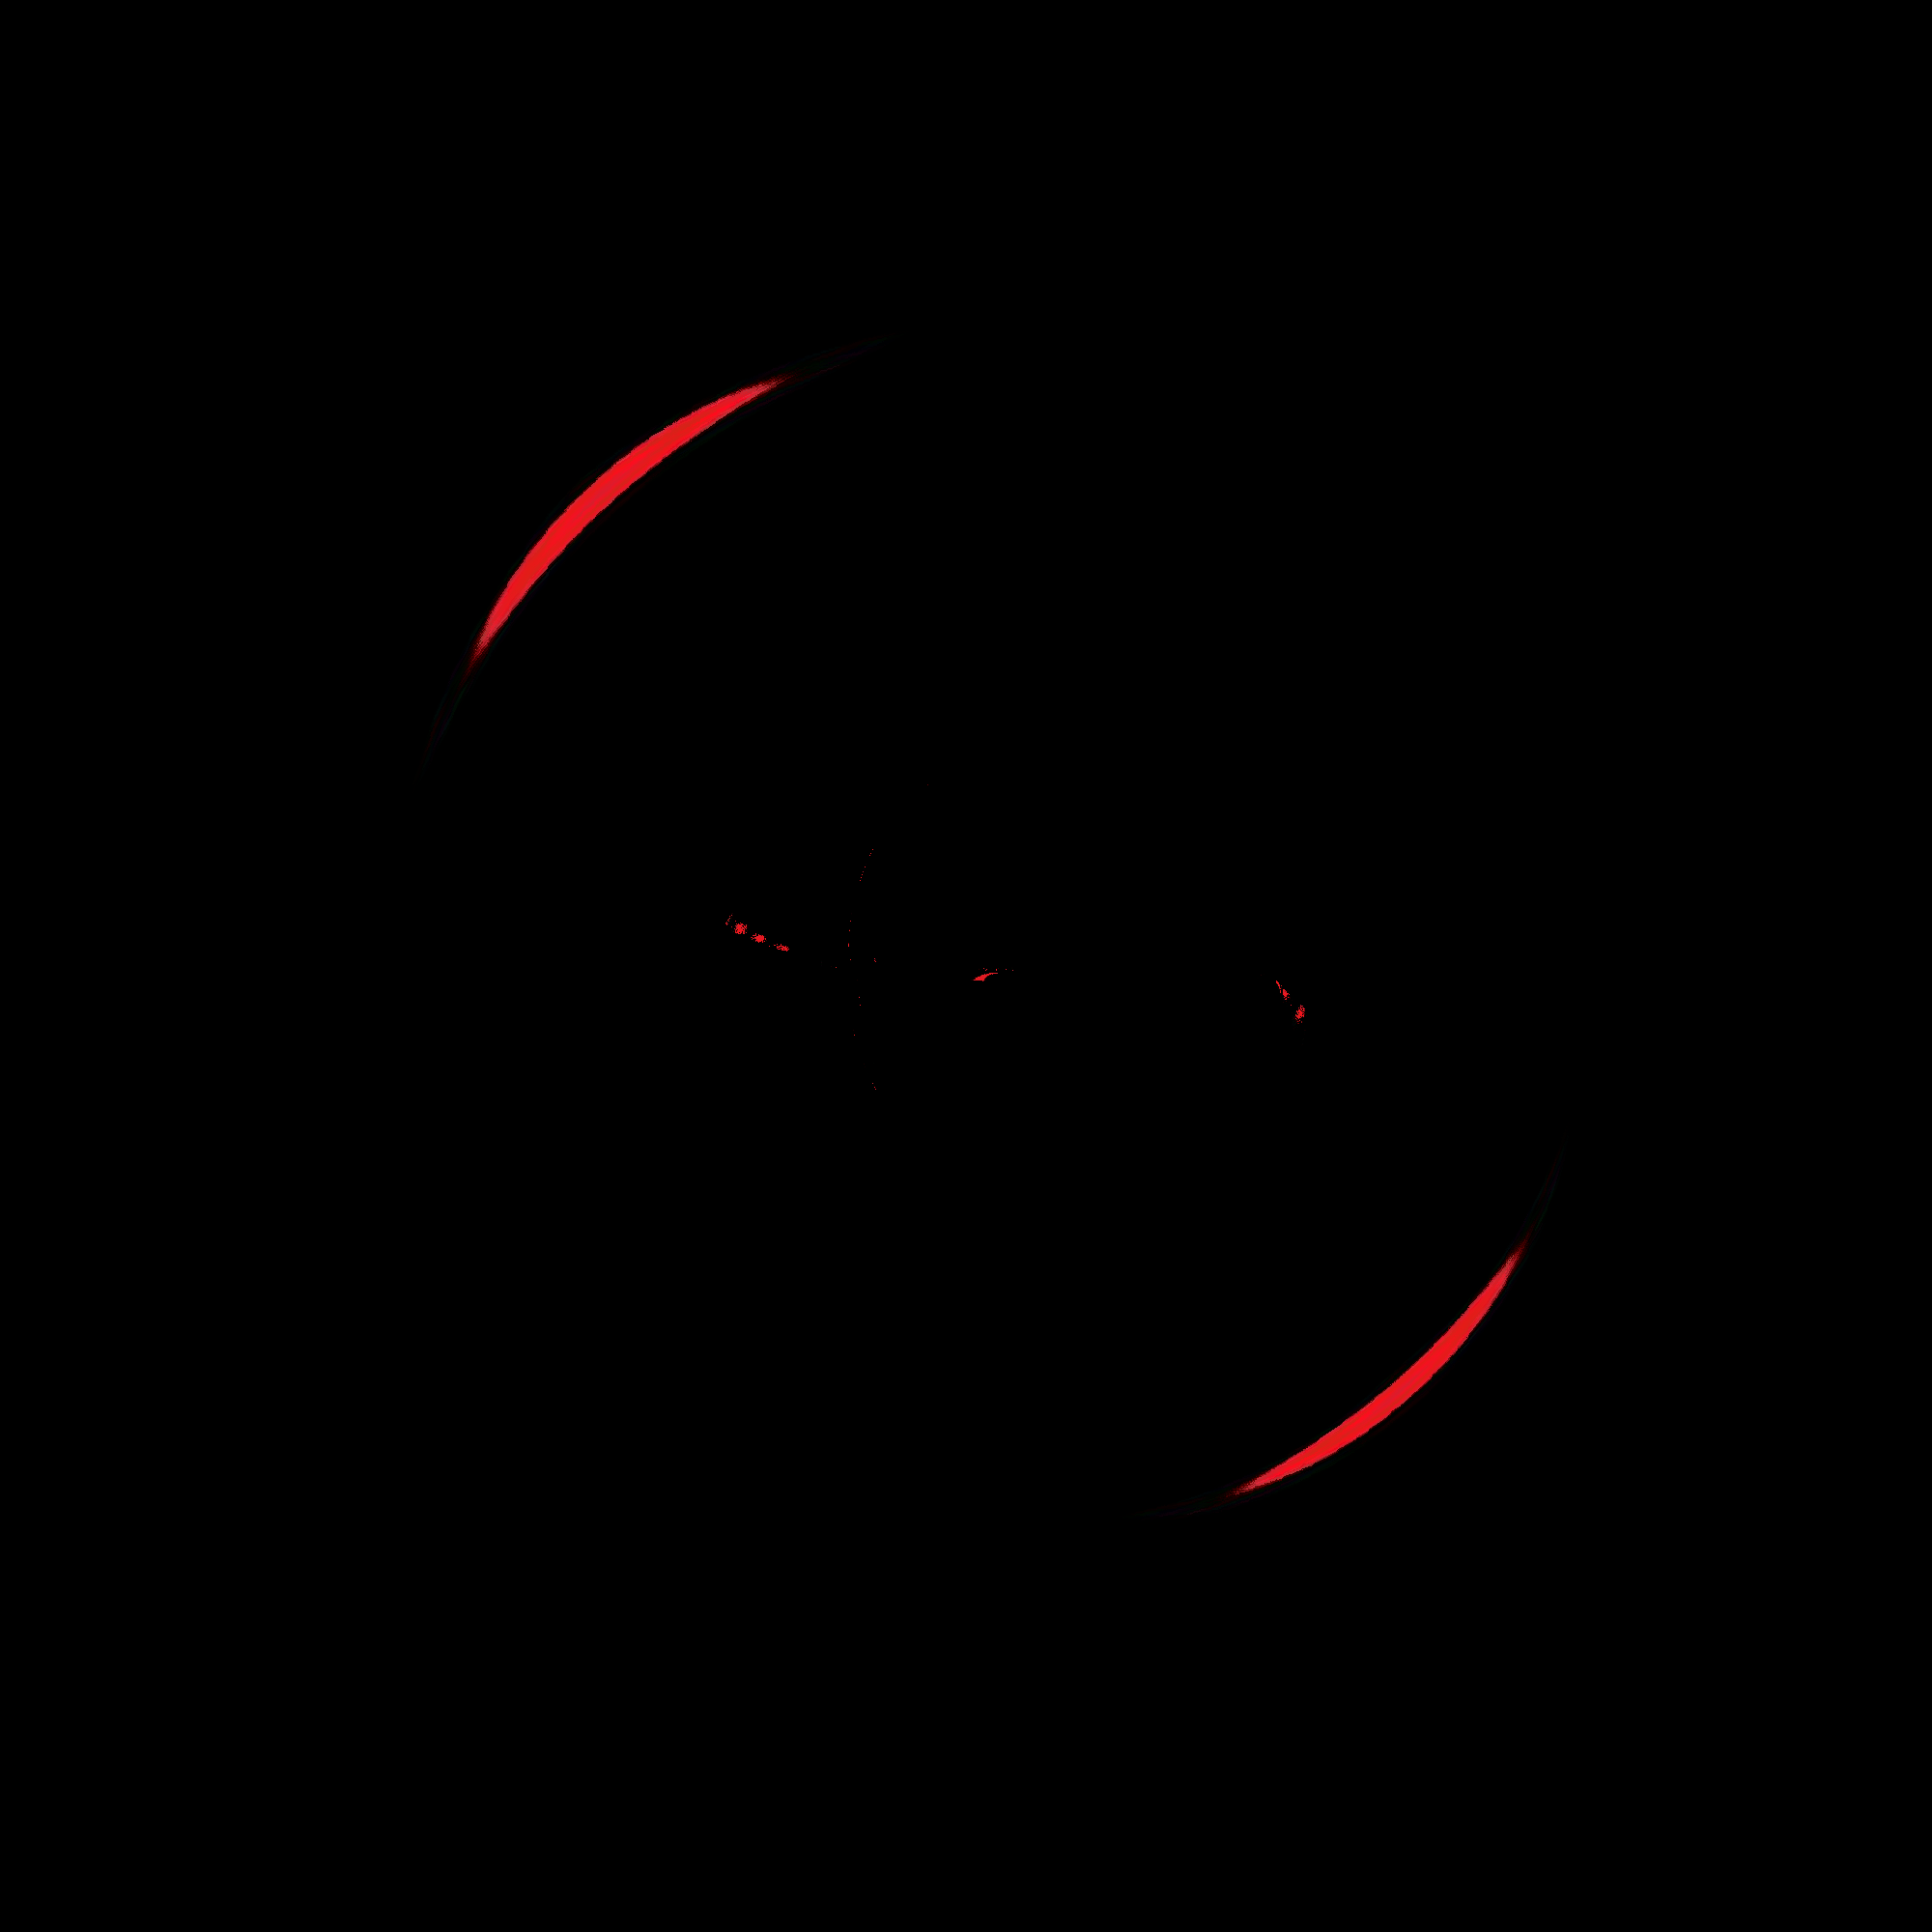
\includegraphics[width=0.6\linewidth]{figures/trace_rad_2000x2000_dot.png} 
    \caption{Gravitational lensing of a point source (red dot) by a near-extremal Kerr black hole ($a=0.998$). The two large crescent arcs represent the primary and secondary images, while the tiny red dots near the center correspond to higher-order photon sub-rings (photons that have orbited the black hole multiple times).}
    \label{fig:point_source_lensing}
\end{figure}

The image clearly exhibits the distinct families of images generated by the strong-field deflection mechanism:

\begin{itemize}
    \item \textbf{Primary and Secondary Images (The Arcs):} The two large, highly magnified crescent arcs located on opposite sides of the shadow correspond to the primary ($n=0$) and secondary ($n=1$) images. These are formed by photons that pass the black hole on either side. The extreme stretching of the originally point-like source into long, thin arcs is a direct consequence of the divergent magnification factor. As the impact parameter approaches the critical curve, the source is stretched tangentially along the boundary of the shadow.
    
    \item \textbf{Higher-Order Sub-rings (The Central Dots):} The tiny red dots clustered near the center of the image, hugging the boundary of the black hole shadow, represent the higher-order images ($n \geq 2$). These are photons that have completed one or more full orbits around the black hole before escaping. 
\end{itemize}

The formation of these higher-order sub-rings is governed by an exponential demagnification process. For a photon to complete an additional loop around the black hole, its initial trajectory must be exponentially closer to the exact critical impact parameter. Consequently, each successive image in the hierarchy is exponentially smaller, fainter, and located exponentially closer to the mathematical shadow boundary than the previous one.

From a computational perspective, resolving these higher-order images represents the ultimate stress test for any relativistic ray-tracing algorithm. Photons that form the central dots spend a significantly long affine parameter time navigating the highly unstable region near the photon sphere. In this region, the Lyapunov exponent of the spacetime dictates that any microscopic numerical error will grow exponentially, artificially ejecting the photon to infinity or causing it to plunge prematurely into the event horizon. 

Standard numerical integrators, which suffer from secular drift in conserved quantities, inevitably smear out or completely erase these higher-order images. The sharp, distinct resolution of the sub-rings in Fig.~\ref{fig:point_source_lensing} provides direct, visual confirmation of the efficacy of our Manifold Projection algorithm. By strictly enforcing the null condition and the conservation of energy and angular momentum at every integration step, our framework suppresses this numerical drift, allowing us to faithfully capture the theoretically predicted infinite hierarchy of photon rings that would otherwise be lost to numerical noise.
\subsection{Shadow Morphology and Frame Dragging}

The mathematical shadow of the black hole is defined by the boundary between the photons that are captured and those that escape.

\begin{figure}[H]
    \centering
    
\includegraphics[width=0.5\linewidth]{figures/trace_rad_2000x2000_test.png}
    \caption{The shadow of the (near-)extremal Kerr black hole (a=0.998) using the calibration image as a celestial sphere.}
    \label{fig:placeholder1}
\end{figure}

Our numerical simulations accurately reproduce the well-known dependence of the shadow morphology on the spin parameter \(a\). For a non-rotating Schwarzschild black hole (\(a = 0\)), the shadow is perfectly circular. As the spin parameter increases towards the extreme Kerr limit (\(a \to 0.998\)), the shadow exhibits a pronounced asymmetry, taking on a characteristic "D" shape. This deformation is a direct consequence of frame-dragging: photons co-rotating with the black hole are pulled closer to the horizon before escaping, thus shifting the critical impact parameter and breaking the equatorial circularity. Our imaging framework naturally captures this transition without any ad-hoc assumptions, purely from the numerical solution of the geodesic equations. This allows us to now use any background image as a celestial sphere and have (more) realistic images.

\begin{figure}[H]
    \centering
    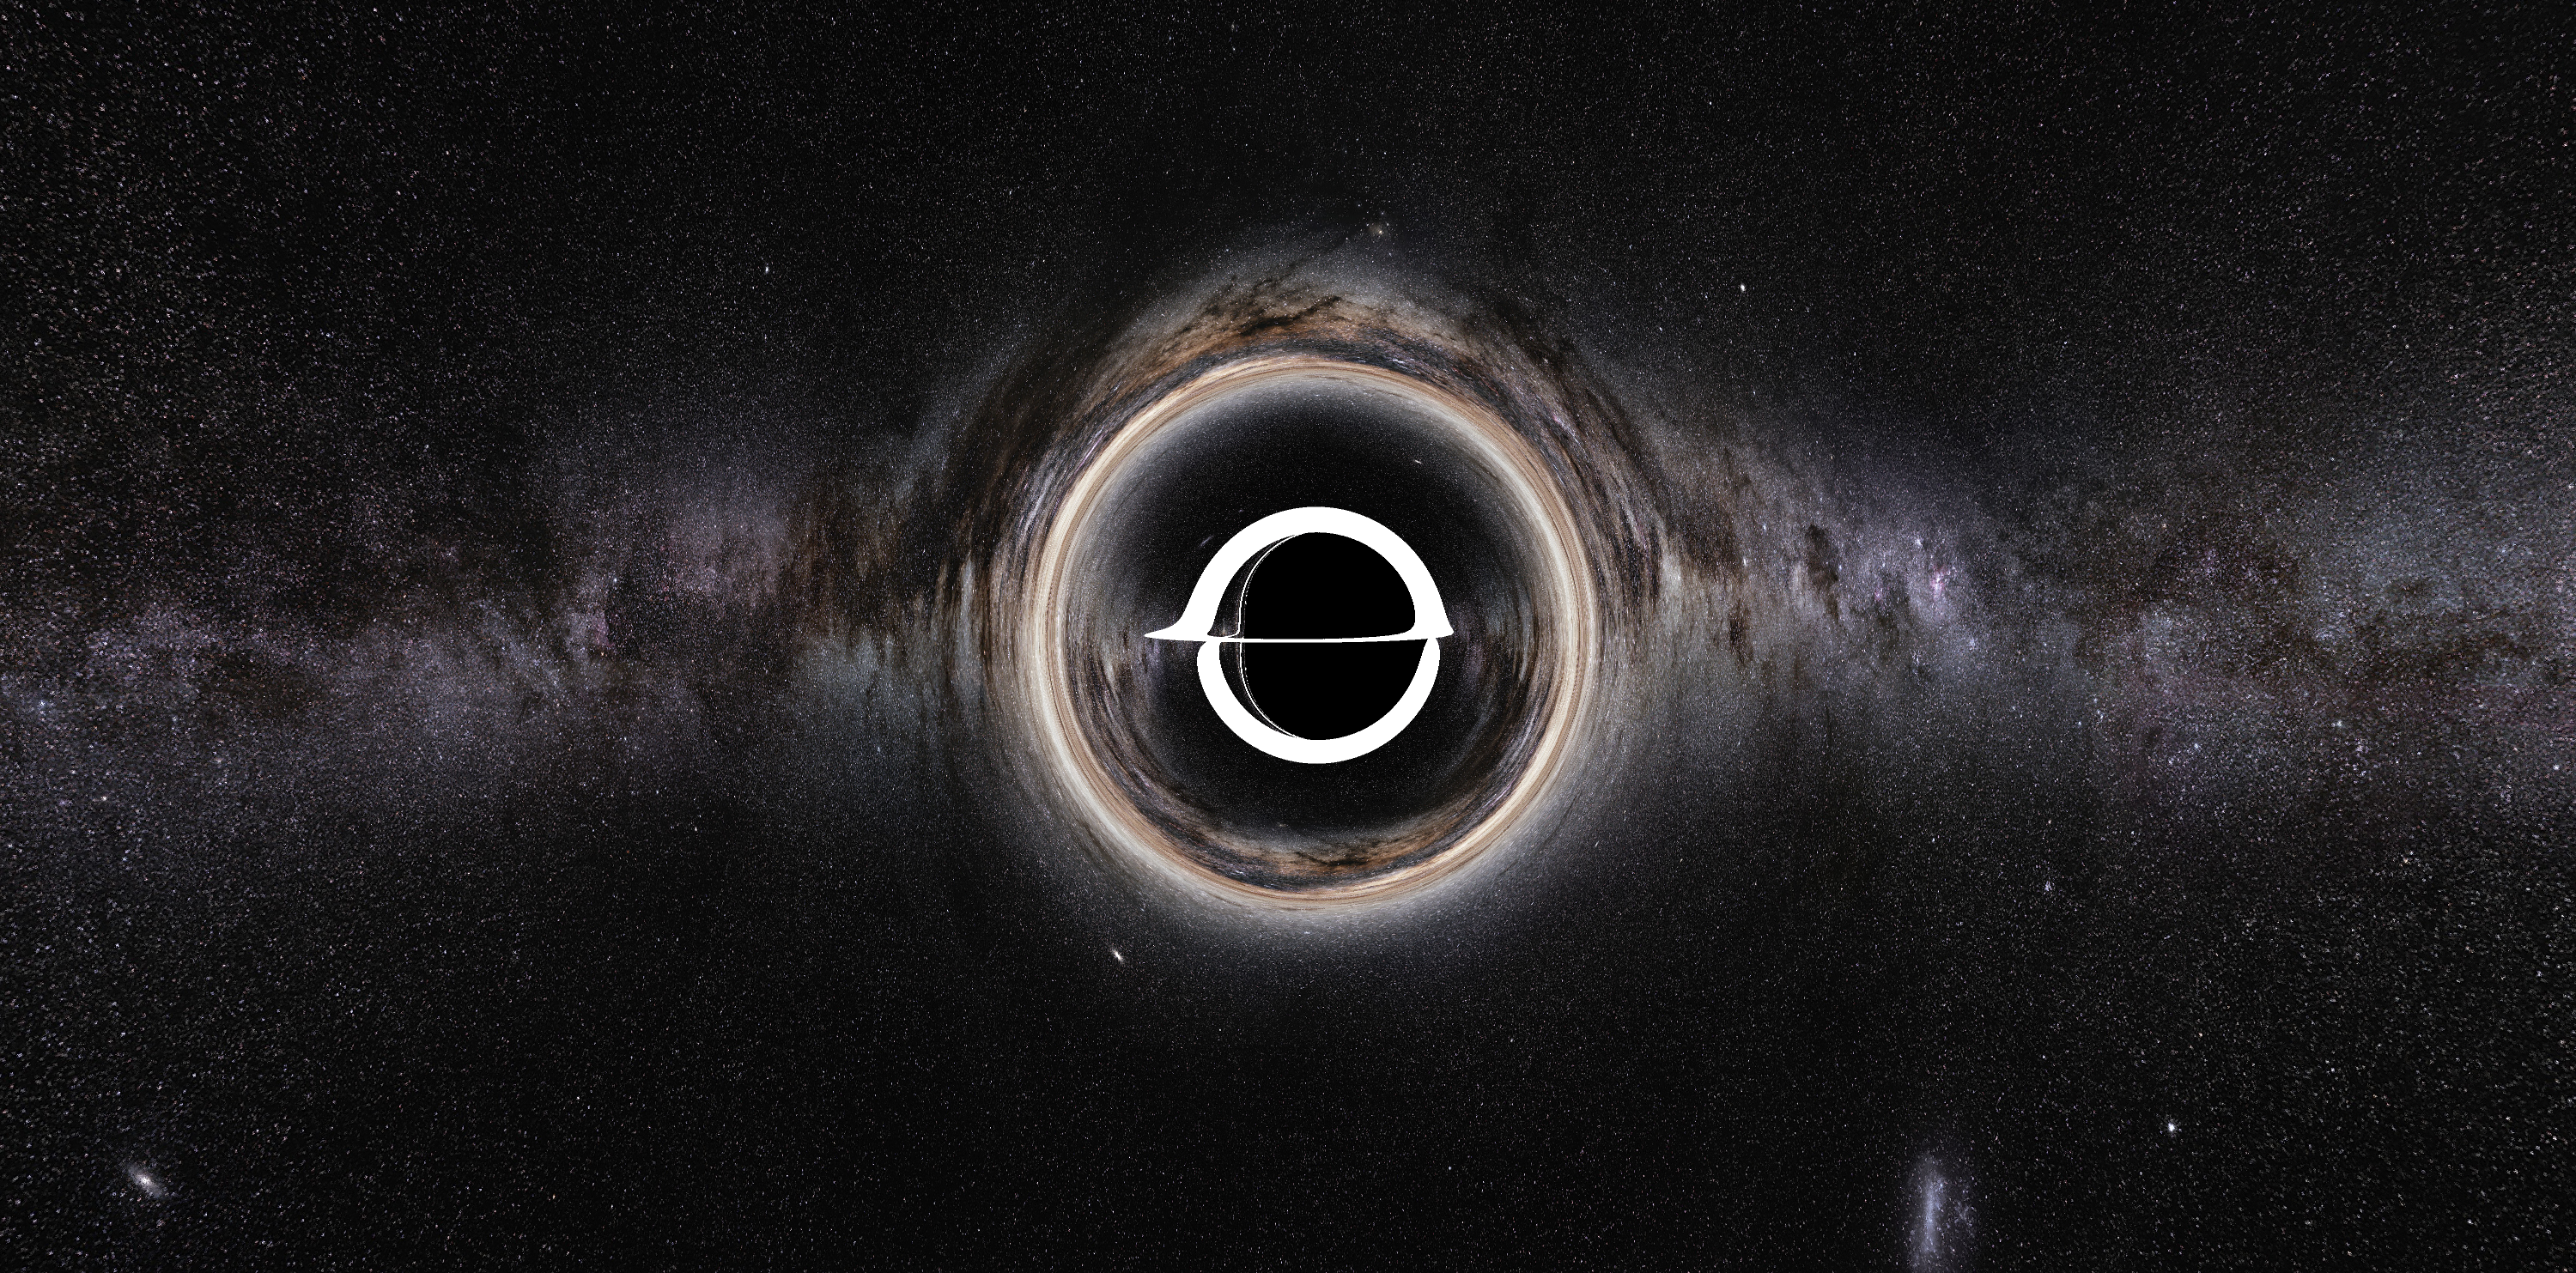
\includegraphics[width=0.75\linewidth]{figures/trace_rad_3000x3000_milky_way(1).png}
    \caption{The shadow of the (near-)extremal Kerr black hole (a=0.998) using the calibration image as a celestial sphere.}
    \label{fig:placeholder}
\end{figure}

\subsection{Relativistic Accretion Disk and Radiative Transfer}

To create astrophysically meaningful images, we extend our framework to include a geometrically thin accretion disk located in the equatorial plane. As described in the theoretical introduction to radiative transfer, the observed intensity \(I_{\text{obs}}\) accumulated along a ray is given by the integral:
\begin{equation}
    I_{\text{obs}} = \int_{\lambda_{\text{source}}}^{\lambda_{\text{obs}}} g^4 \, \epsilon(r) \, d\lambda,
\end{equation}
where \(g\) is the relativistic redshift factor and \(\epsilon(r)\) is the local rest-frame emissivity modelled by our exponential density profile.

The resulting images, presented in Fig.~\ref{fig:disk_images}, highlight several key relativistic phenomena:
\begin{enumerate}
    \item \textbf{Doppler Beaming:} The approaching side of the disk (where the plasma rotates towards the observer) is strongly boosted in intensity, appearing much brighter than the receding side. This asymmetric brightness distribution is a direct consequence of the \(g^4\) scaling.
    \item \textbf{Gravitational Lensing:} The light from the far side of the disk is bent over and under the black hole, forming a narrow, bright photon ring that closely traces the mathematical shadow.
    \item \textbf{Higher-Order Sub-rings:} The photons that wind multiple times around the black hole (as explored in the spiral orbit analysis of Section 3.2) create an infinite hierarchy of sub-rings. Due to our rigorous geometric projection, these sub-rings are resolved with exceptional sharpness, faithfully reproducing the predicted exponential demagnification.
\end{enumerate}

To explicitly visualize the impact of the spin parameter $a$ on the spacetime geometry within a realistic astrophysical context, we contrast the emission from an accretion disk around a non-rotating Schwarzschild black hole ($a=0$) with that of a near-extremal Kerr black hole ($a=0.998$). 

\begin{figure}[H]
    \centering
    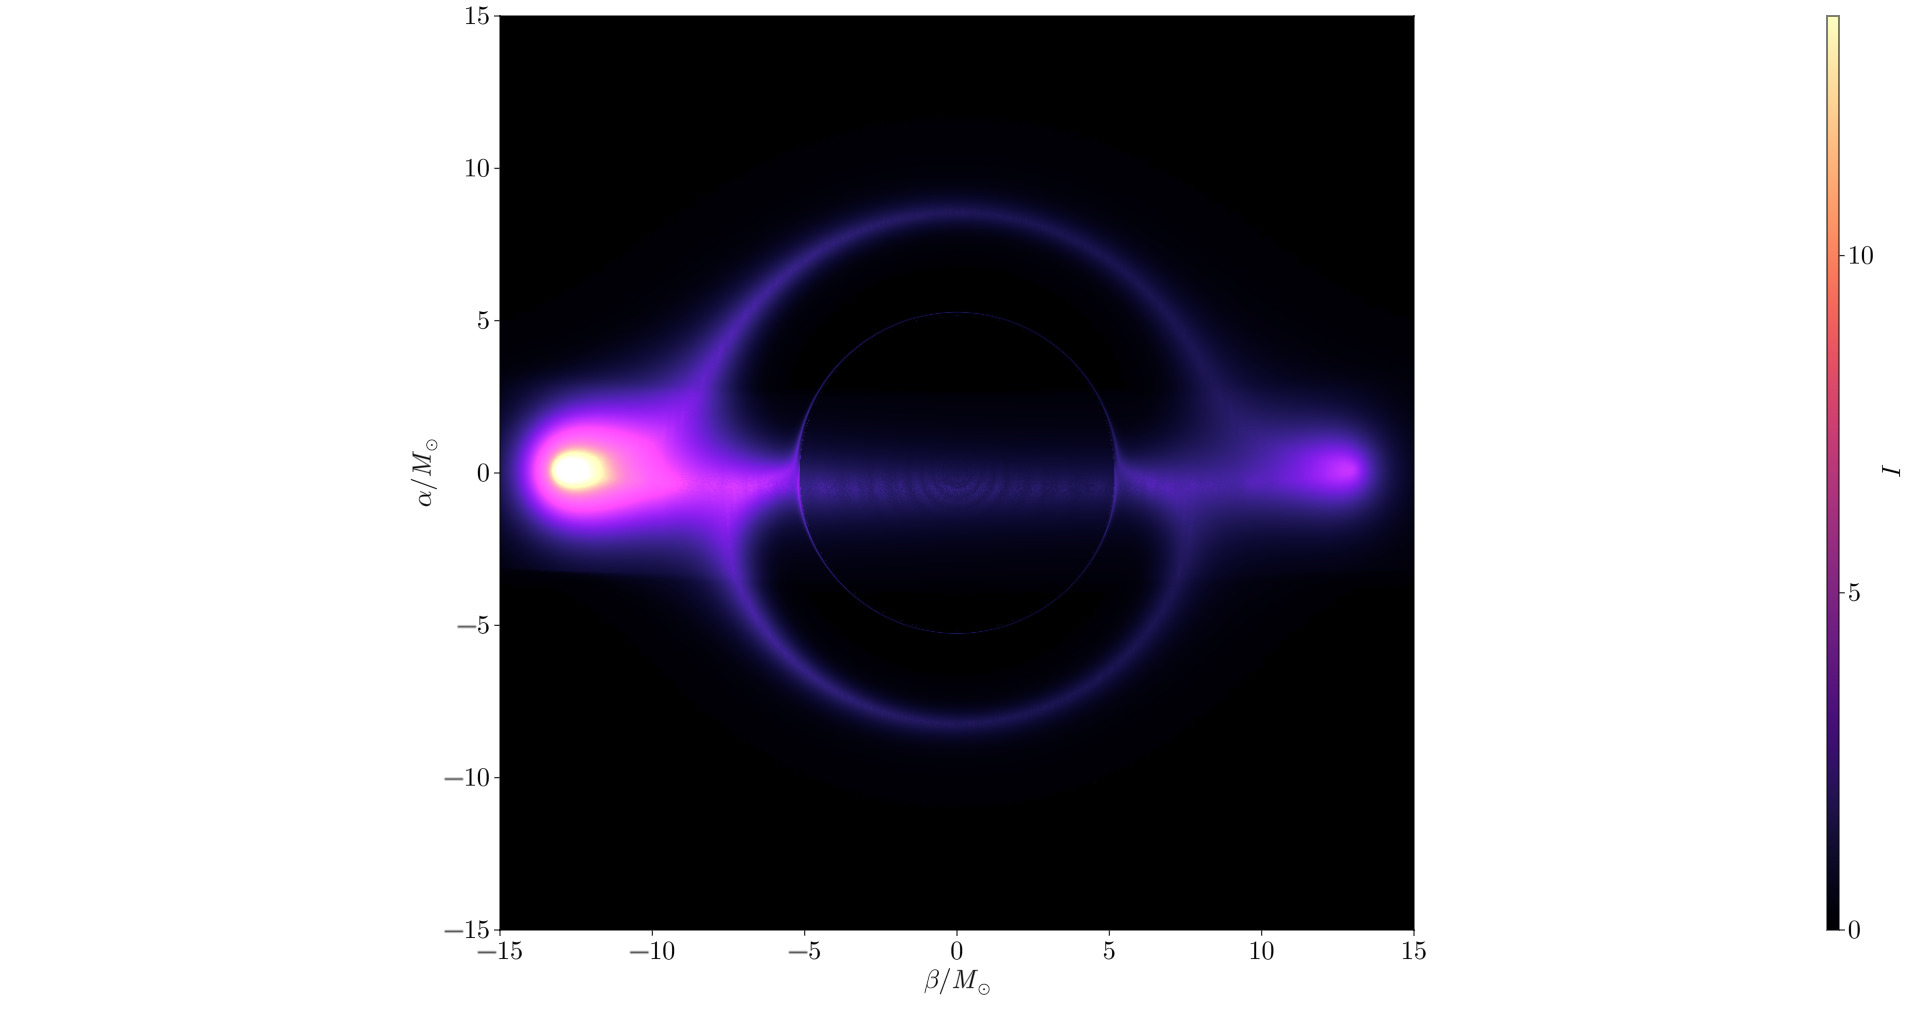
\includegraphics[width=1.0\textwidth]{figures/bh_shadow_1000x1000_a000.png}
    \caption{Relativistic accretion disk around a non-rotating Schwarzschild black hole ($a=0$). While the asymmetric brightness due to Doppler beaming is still present, the central mathematical shadow remains a perfect circle, directly contrasting with the deformed "D" shape of the Kerr metric.}
    \label{fig:disk_schwarzschild}
\end{figure}

As shown in Fig.~\ref{fig:disk_schwarzschild}, in the absence of frame-dragging, the mathematical shadow bounded by the photon ring remains perfectly circular. While the kinematic Doppler beaming still causes a strong left-right brightness asymmetry in the accretion disk, the underlying geometric boundary of the photon capture region is strictly isotropic. In stark contrast, Fig.~\ref{fig:disk_image} demonstrates how the extreme rotation of the Kerr spacetime drags the surrounding geometry, compressing the photon ring on the co-rotating side and elongating it on the counter-rotating side, thereby manifesting the characteristic "D" shape.

\begin{figure}[H]
    \centering
    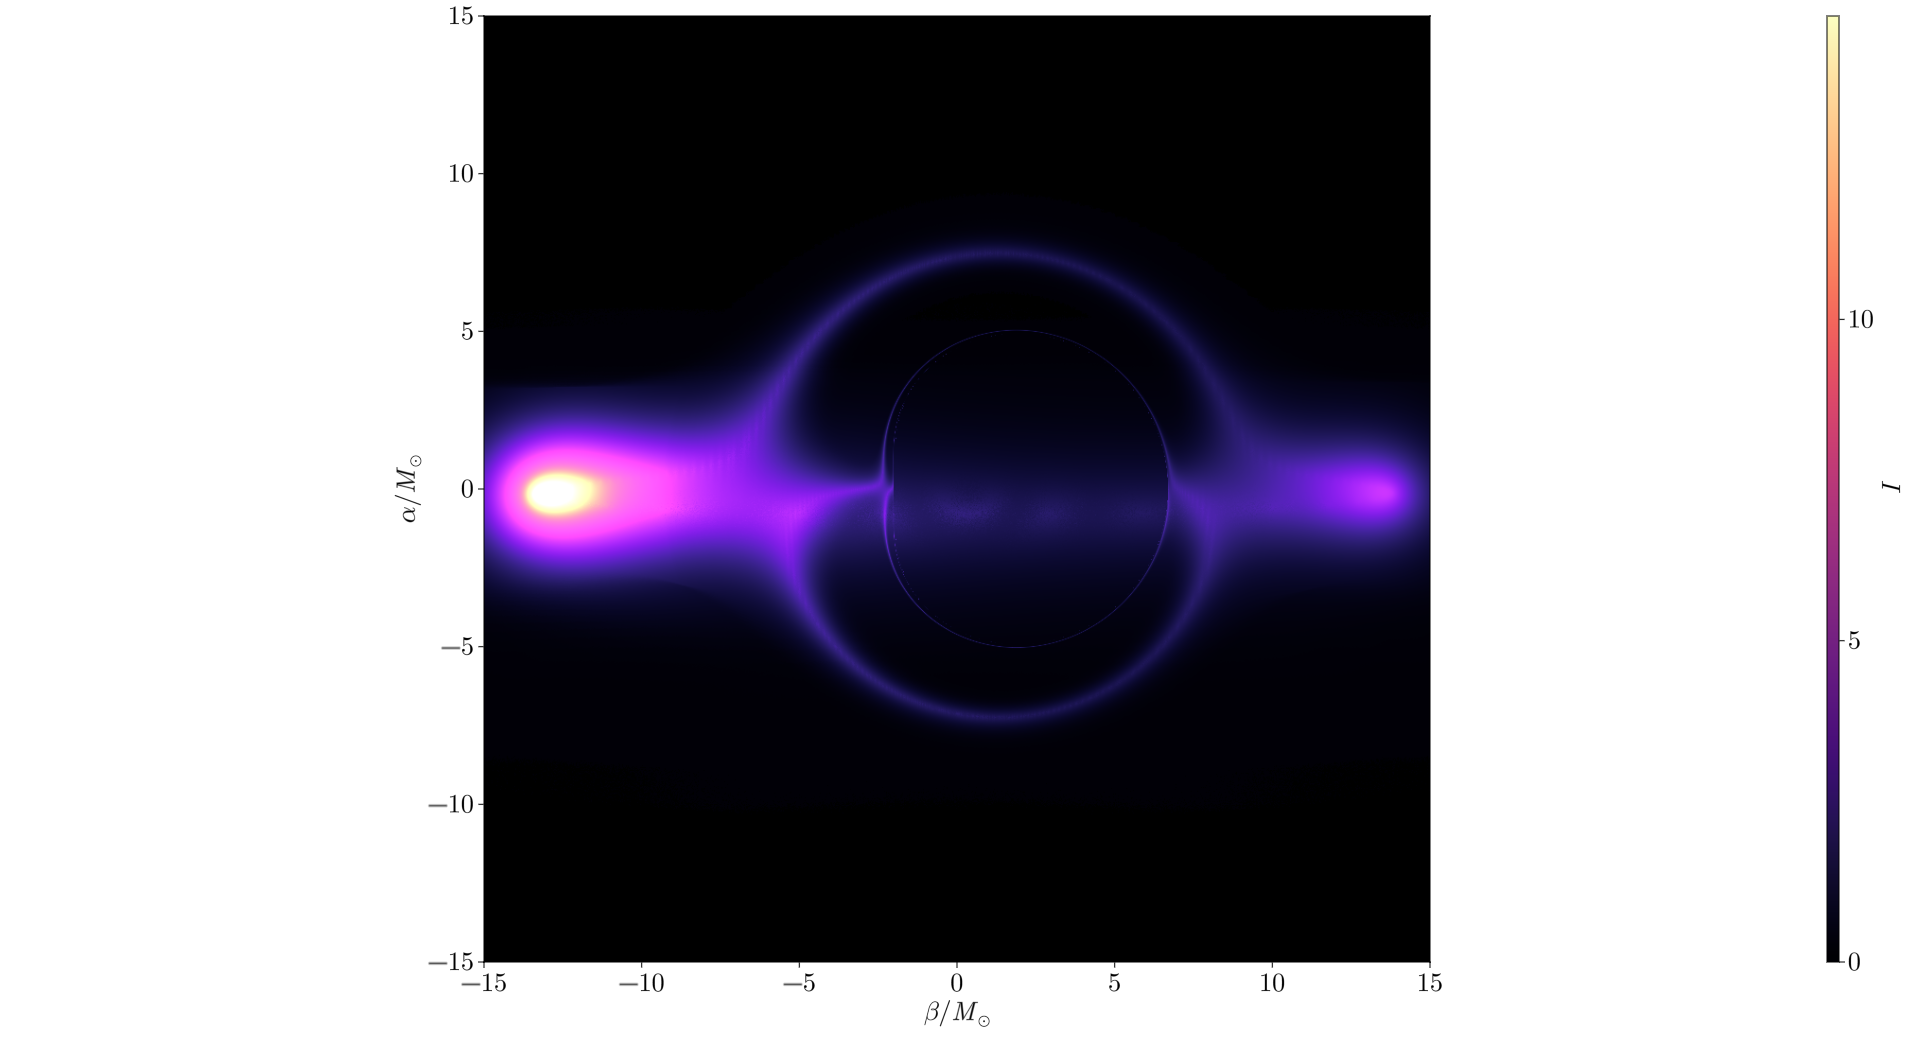
\includegraphics[width=1.0\textwidth]{figures/bh_shadow_1000x1000.png}
    \caption{Thin disk accretion disk around a Kerr black hole ($a=0.998)$.}
    \label{fig:disk_image}
\end{figure}

The combination of an (near)-extremal Kerr geometry, relativistic Doppler beaming, and a realistic background demonstrates the full capability of our framework. These images not only serve as powerful visual tools for understanding strong-field gravity, but also provide a robust, numerically accurate platform for interpreting the horizon-scale observations from current and future interferometric campaigns such as the Event Horizon Telescope (EHT).

\begin{figure}[H]
    \centering
    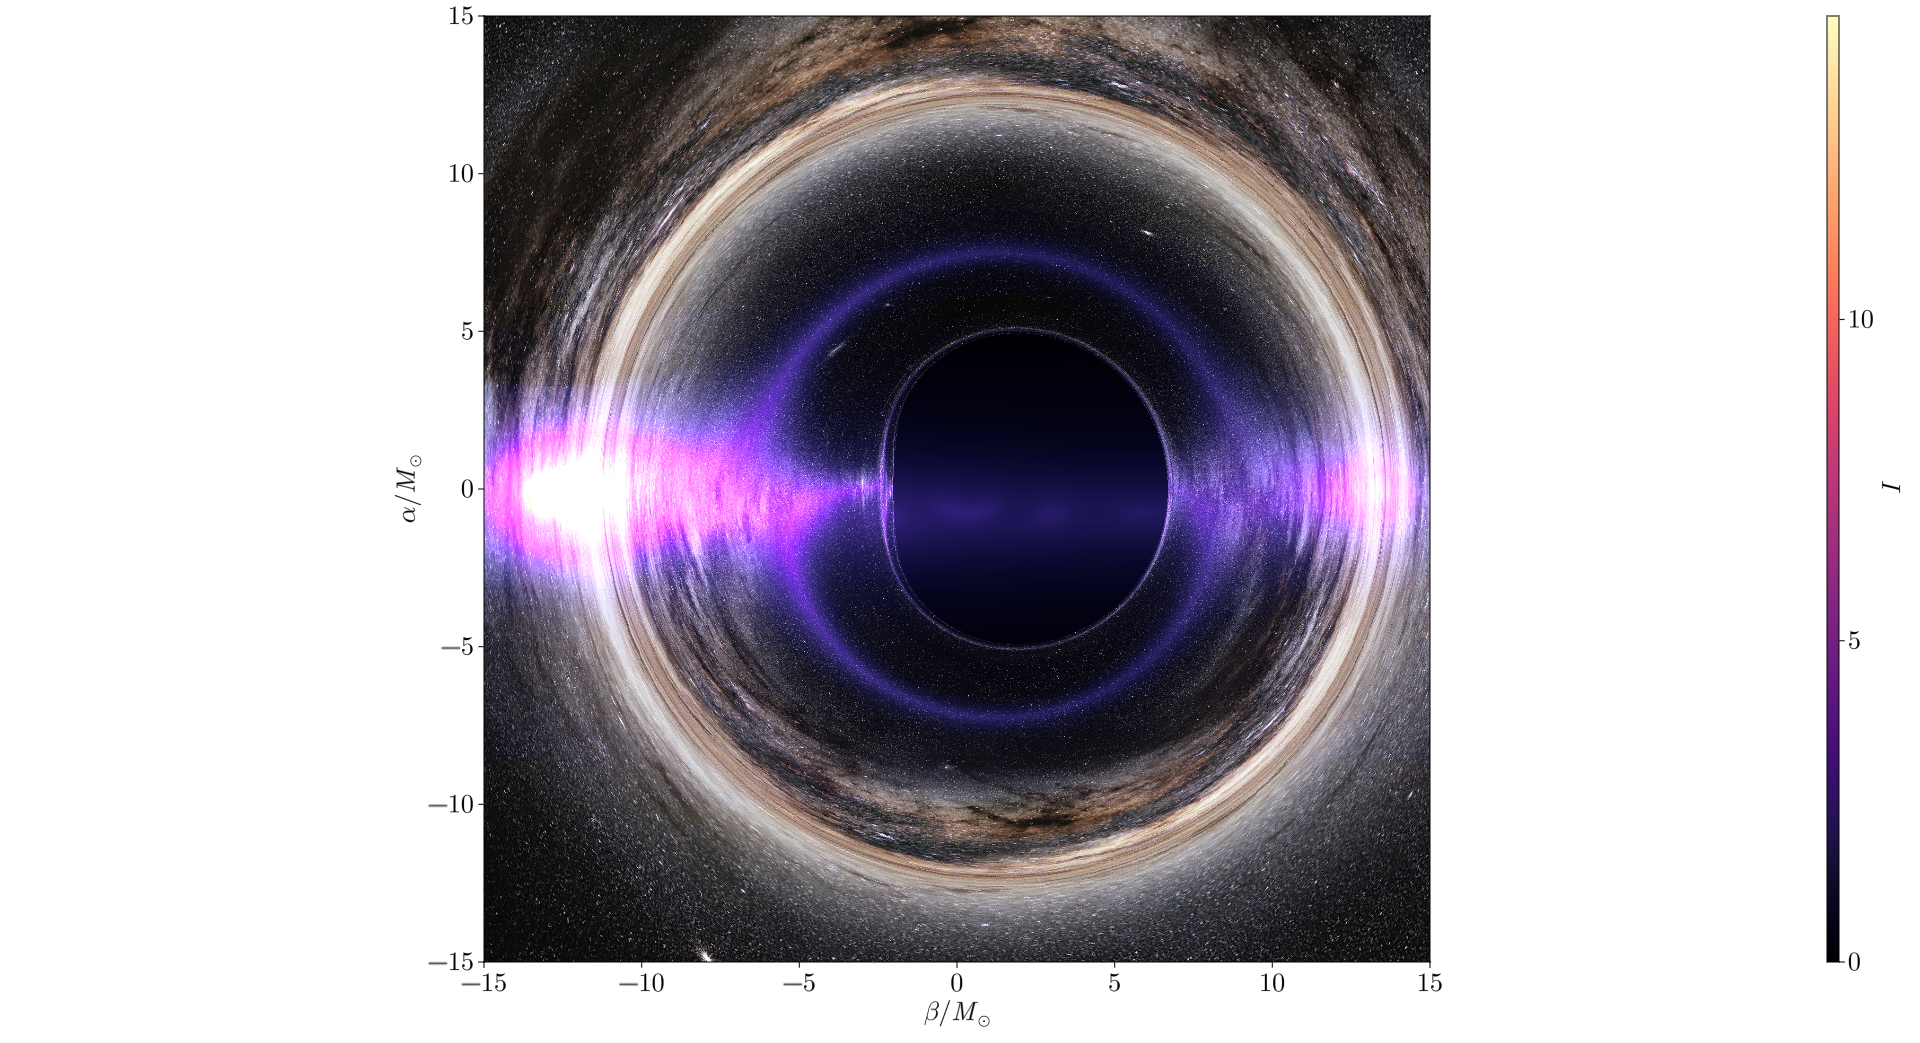
\includegraphics[width=0.8\textwidth]{figures/thin_disk_2000x2000_milky_way.png}
    \caption{Thin disk accretion disk around a Kerr black hole ($a=0.998)$, with a realistic (Milky Way) celestial sphere.}
    \label{fig:disk_images}
\end{figure}


\chapter{Conclusions and Future Prospects}

\section{Summary of Contributions}

In this thesis, we have developed, implemented, and validated a robust computational framework for the numerical simulation and visualization of relativistic ray tracing in the strong-field regime of rotating Kerr black holes. Motivated by the recent observational breakthroughs of the Event Horizon Telescope (EHT), our work addresses the fundamental challenge of generating high-fidelity synthetic images, which requires tracing millions of photon trajectories through an environment characterized by extreme numerical sensitivity and chaotic dynamics.

The core methodological achievement of this work lies in the synthesis of two advanced computational techniques designed to overcome the limitations of traditional numerical relativity codes. First, to address the bottleneck of computing exact metric derivatives and Christoffel symbols, we implemented Forward-Mode Automatic Differentiation (AD). By extending the arithmetic of the Julia programming language, we completely eliminated the truncation and round-off errors inherent to finite difference methods. This approach not only guarantees derivatives to machine precision ($\sim 10^{-16}$) but also renders the framework entirely metric-agnostic, allowing it to be applied to any spacetime geometry without manual algebraic derivation.

Second, to mitigate the severe invariant drift exhibited by standard explicit Runge-Kutta integrators near the unstable photon sphere, we coupled a high-order adaptive integrator with a geometric Manifold Projection algorithm. By formulating the physical constraints—the null condition, energy conservation, and axial angular momentum conservation—as a constraint manifold $\mathcal{N}$, we employed Lagrange multipliers and a multidimensional Newton-Raphson solver to project the numerical state back onto $\mathcal{N}$ at every integration step. Crucially, this correction is strictly orthogonal to the physical flow, ensuring that the trajectory is stabilized without introducing artificial numerical damping.

We systematically validated the numerical stability of this framework across the three fundamental classes of photon orbits: scattering, direct capture, and bound spirals. In all regimes, particularly for the highly chaotic transient capture orbits, the framework successfully maintained conserved quantities at the machine-precision limit. This exceptional numerical fidelity enabled the resolution of the infinite hierarchy of higher-order photon sub-rings—a feature typically smeared out or entirely lost by standard numerical methods due to secular drift.

Applying this framework to astrophysical imaging, we successfully reproduced the characteristic asymmetric ``D-shaped'' shadow of a near-extremal Kerr black hole ($a=0.998$) induced by frame-dragging. Through rigorous UV mapping calibration using a four-color test image, we ensured physically accurate lensing of realistic backgrounds, such as the Milky Way. Furthermore, by incorporating a geometrically thin accretion disk model with relativistic radiative transfer ($I \propto g^4$), we captured key observable phenomena, including extreme Doppler beaming and the complex gravitational lensing of the disk's far side. Beyond accuracy, the framework is highly efficient; on a standard 16-core laptop, it processes computationally demanding trajectories at an average rate of one million rays per hour, making it a practical tool for large-scale parameter space exploration.

\section{Future Research Directions}

The computational infrastructure developed in this thesis lays the groundwork for several promising research extensions. The metric-agnostic architecture, the machine-precision conservation of invariants, and the high performance of the framework make it a versatile platform that can be expanded in multiple directions relevant to next-generation observational astrophysics.

\subsection{GPU Acceleration and Real-Time Rendering}

While the current CPU multi-threaded implementation achieves a throughput of approximately one million rays per hour on a standard 16-core laptop, the embarrassingly parallel nature of backward ray tracing makes it an ideal candidate for massive parallelization on Graphics Processing Units (GPUs). Each pixel on the observer's screen corresponds to an independent initial value problem, meaning that millions of geodesics can be integrated simultaneously without inter-thread communication overhead.

Porting the inner geodesic and projection kernels to GPUs would reduce the rendering time from hours to seconds, enabling real-time visualization of black hole shadows at high resolution. This capability would be particularly valuable for interactive scientific exploration, educational purposes, and the rapid generation of large datasets required for machine learning applications. Furthermore, GPU acceleration would make feasible the computation of time-dependent images from dynamical spacetimes, such as those arising from binary black hole mergers or accretion disk instabilities.

\subsection{Extension to Alternative Metrics and Beyond-GR Theories}

One of the most significant advantages of the framework is its metric-agnostic nature, stemming from the use of Automatic Differentiation to compute Christoffel symbols. This feature allows the code to be applied to any spacetime geometry without requiring manual algebraic derivation of connection coefficients, making it an ideal tool for testing alternative theories of gravity.
By systematically comparing the synthetic images produced by these alternative metrics with observational data from the Event Horizon Telescope (EHT) and its next-generation upgrade (ngEHT), one could place quantitative constraints on deviations from General Relativity in the strong-field regime.

\subsection{Template Generation and Parameter Estimation}

The high fidelity and computational efficiency of the framework make it well-suited for the generation of large libraries of synthetic images (templates) that can be used in Bayesian parameter estimation pipelines. Current EHT analyses rely on comparing observed interferometric visibilities with pre-computed template libraries generated by general relativistic magnetohydrodynamic (GRMHD) simulations coupled with ray-tracing codes.\\
By integrating the forward ray-tracer with differentiable programming techniques, one could construct a fully differentiable imaging pipeline in which the synthetic image is a differentiable function of the black hole parameters (mass $M$, spin $a$, inclination $\theta_0$, accretion rate, etc.).\\
Such a differentiable pipeline would represent a significant advancement in the analysis of horizon-scale observations, bridging the gap between theoretical predictions and observational data in a computationally efficient and statistically rigorous manner.
\newpage

\bibliographystyle{abbrv}
\bibliography{bib}

\end{document}

\bibliographystyle{plain}
\begin{thebibliography}{99}

\bibitem{Bardeen1973}
J.~M.~Bardeen.
\newblock Timelike and null geodesics in the {Kerr} metric.
\newblock {\em Black Holes (Les Astres Occlus)}, pages 215--240, 1973.

\bibitem{Carter1968}
B.~Carter.
\newblock Global structure of the {Kerr} family of gravitational fields.
\newblock {\em Physical Review}, 174(5):1559--1571, 1968.

\bibitem{EHT2019}
Event Horizon~Telescope Collaboration.
\newblock First {M87} {Event} {Horizon} {Telescope} results. {I}. {The} shadow of the supermassive black hole.
\newblock {\em The Astrophysical Journal Letters}, 875(1):L1, 2019.

\bibitem{Gralla2019}
S.~E.~Gralla, D.~E.~Holz, and R.~M.~Wald.
\newblock Black hole shadows, photon rings, and lensing rings.
\newblock {\em Physical Review D}, 100(2):024018, 2019.

\bibitem{Hairer2006}
E.~Hairer, C.~Lubich, and G.~Wanner.
\newblock {\em Geometric Numerical Integration: Structure-Preserving Algorithms for Ordinary Differential Equations}.
\newblock Springer Science \& Business Media, 2nd edition, 2006.

\bibitem{Revels2016}
J.~Revels, M.~Lubin, and T.~Papamarkou.
\newblock {Forward-Mode} automatic differentiation in {Julia}.
\newblock {\em arXiv preprint arXiv:1607.07892}, 2016.

\bibitem{Younsi2012}
Z.~Younsi, K.~Wu, and S.~V.~Fuerst.
\newblock General relativistic radiative transfer: formulation and emission from structured tori around black holes.
\newblock {\em Astronomy \& Astrophysics}, 545:A13, 2012.

\end{thebibliography}

\end{document}